% !TEX program = xelatex
\documentclass[UTF8,fontset=fandol,a4paper,11pt]{ctexart}
\usepackage[margin=21mm,top=23mm,bottom=22mm,headheight=16pt]{geometry}
\usepackage{amsmath,amssymb,mathtools,bm}
\usepackage{tikz}
\usetikzlibrary{arrows.meta,calc,angles,quotes,patterns}
\usepackage{xcolor,booktabs,array,longtable,enumitem,fancyhdr,needspace}
\usepackage[unicode,hidelinks]{hyperref}
\definecolor{ink}{HTML}{24343C}
\definecolor{accent}{HTML}{166A70}
\definecolor{muted}{HTML}{65747A}
\definecolor{rulegray}{HTML}{D4DDE0}
\definecolor{warm}{HTML}{966037}
\color{ink}
\setlength{\parindent}{2em}
\setlength{\parskip}{4pt}
\linespread{1.12}
\AtBeginDocument{\setlength{\abovedisplayskip}{6pt plus 2pt minus 1pt}
\setlength{\belowdisplayskip}{6pt plus 2pt minus 1pt}
\setlength{\abovedisplayshortskip}{0pt plus 1pt}
\setlength{\belowdisplayshortskip}{4pt plus 1pt}}
\setlist[enumerate]{label=(\arabic*),leftmargin=2.3em,itemsep=3pt,topsep=4pt}
\setlist[itemize]{leftmargin=2em,itemsep=2pt,topsep=4pt}
\allowdisplaybreaks[1]
\setlength{\emergencystretch}{2em}
\setcounter{secnumdepth}{0}
\providecommand{\tightlist}{\setlength{\itemsep}{0pt}\setlength{\parskip}{0pt}}
\ctexset{section={format=\Large\bfseries\color{accent},beforeskip=10pt,afterskip=9pt},
subsection={format=\normalsize\bfseries\color{accent},beforeskip=10pt,afterskip=4pt},
subsubsection={format=\normalsize\bfseries,beforeskip=8pt,afterskip=3pt}}
\pagestyle{fancy}
\fancyhf{}
\fancyhead[L]{\small\color{muted}物理学难题集萃}
% 页眉仅保留书名；版本名称只在封面显示。
\fancyfoot[L]{\small\color{muted}\chapterlabel}
\fancyfoot[R]{\small\thepage}
\renewcommand{\headrulewidth}{0.4pt}
\renewcommand{\footrulewidth}{0pt}
\newcommand{\dd}{\mathop{}\!\mathrm{d}}
\newcommand{\vect}[1]{\bm{#1}}
\newcommand{\tagline}[1]{\noindent{\small\color{muted}#1}\par}
\newcommand{\result}[1]{\begin{equation*}\boxed{#1}\end{equation*}}
\newcommand{\figcaption}[1]{\par\vspace{2pt}{\small\color{muted}#1}\par}
\newcommand{\teach}[2]{\Needspace{4\baselineskip}\subsection*{讲解要点与追问}#1\par\smallskip\noindent\textbf{追问：}#2\par}
\newcommand{\workarea}{\par\vspace{7mm}\noindent{\small\color{muted}作答区}\par\vspace{4mm}
\noindent\textcolor{rulegray}{\rule{\linewidth}{0.3pt}}\par\vspace{16mm}
\noindent\textcolor{rulegray}{\rule{\linewidth}{0.3pt}}\par\vspace{16mm}
\noindent\textcolor{rulegray}{\rule{\linewidth}{0.3pt}}\par\vspace{16mm}
\noindent\textcolor{rulegray}{\rule{\linewidth}{0.3pt}}}
\tikzset{axis/.style={-{Stealth[length=2mm]},thin,color=muted},
motion/.style={-{Stealth[length=2.3mm]},thick,color=accent},
force/.style={-{Stealth[length=2.3mm]},thick,color=warm},
traj/.style={thick,color=accent},guide/.style={dashed,thin,color=muted},
object/.style={thick,color=ink},every node/.style={font=\small}}\widowpenalty=10000\clubpenalty=10000\displaywidowpenalty=10000\newcommand{\chapterlabel}{近代物理第二章\quad 狭义相对论}







\hypersetup{pdftitle={近代物理第二章 狭义相对论·学生版},pdfauthor={}}

\begin{document}\pdfbookmark[0]{近代物理第二章 狭义相对论}{cover}

\thispagestyle{empty}\vspace*{22mm}

\noindent{\Huge\bfseries 物理学难题集萃}\par\vspace{10mm}

\noindent{\LARGE 近代物理第二章}\par\vspace{6mm}

\noindent{\LARGE 狭义相对论}\par\vspace{12mm}

\noindent{\Large\color{accent}学生版}\par\vspace{9mm}

\noindent\textcolor{accent}{\rule{\linewidth}{1pt}}\par\vspace{9mm}

\noindent 第1--19题\par\vfill\clearpage

\pdfbookmark[1]{题目目录}{contents}\section*{题目目录}

\begin{longtable}{@{}r p{113mm} r@{}}\toprule 题号 & 题目 & 页码\\\midrule

\hyperref[q:1]{1} & \hyperref[q:1]{飞船、定站与往返信号} & \pageref{q:1} \\

\hyperref[q:2]{2} & \hyperref[q:2]{运动中性线框的电荷与电偶极} & \pageref{q:2} \\

\hyperref[q:3]{3} & \hyperref[q:3]{两艘相向飞船的光信号} & \pageref{q:3} \\

\hyperref[q:4]{4} & \hyperref[q:4]{沿法线运动的平面镜} & \pageref{q:4} \\

\hyperref[q:5]{5} & \hyperref[q:5]{共同运动的介质界面} & \pageref{q:5} \\

\hyperref[q:6]{6} & \hyperref[q:6]{运动观察者所见的星空分布} & \pageref{q:6} \\

\hyperref[q:7]{7} & \hyperref[q:7]{运动点光源的接收强度} & \pageref{q:7} \\

\hyperref[q:8]{8} & \hyperref[q:8]{迎面反射镜返回的光功率} & \pageref{q:8} \\

\hyperref[q:9]{9} & \hyperref[q:9]{移动色散介质中的相速度} & \pageref{q:9} \\

\hyperref[q:10]{10} & \hyperref[q:10]{固有加速度恒定的星际航程} & \pageref{q:10} \\

\hyperref[q:11]{11} & \hyperref[q:11]{相对论火箭的质量比} & \pageref{q:11} \\

\hyperref[q:12]{12} & \hyperref[q:12]{光子火箭的巡航速度与燃料下限} & \pageref{q:12} \\

\hyperref[q:13]{13} & \hyperref[q:13]{恒固有加速度光子火箭的初始功率} & \pageref{q:13} \\

\hyperref[q:14]{14} & \hyperref[q:14]{高空缪子的寿命与磁偏转} & \pageref{q:14} \\

\hyperref[q:15]{15} & \hyperref[q:15]{电子与质子在非均匀磁场中的同轨运动} & \pageref{q:15} \\

\hyperref[q:16]{16} & \hyperref[q:16]{横向恒力作用下的相对论粒子} & \pageref{q:16} \\

\hyperref[q:17]{17} & \hyperref[q:17]{极端相对论粒子与双夸克模型} & \pageref{q:17} \\

\hyperref[q:18]{18} & \hyperref[q:18]{引力束缚尺度与模型的适用范围} & \pageref{q:18} \\

\hyperref[q:19]{19} & \hyperref[q:19]{引力红移、恒星参数与离子反冲} & \pageref{q:19} \\

\bottomrule\end{longtable}

\clearpage

\pdfbookmark[2]{第 1 题 飞船、定站与往返信号}{q1}

\section*{第 1 题\quad 飞船、定站与往返信号}\label{q:1}

一艘飞船以$0.8c$沿直线飞离地球。飞船中午经过地球时，船钟与地球钟均调为12:00。沿航向有一座相对地球静止的定站，站钟与地球钟按地球惯性系同步。船钟12:30时，飞船经过定站，并立即向地球发射无线电信号。
\begin{enumerate}
\item 飞船经过定站时，站钟读数是多少？
\item 地球系测得地球至定站的距离是多少？
\item 地球何时接收到信号？
\item 地球接收后立即回信。飞船保持匀速，何时按船钟接收到回信？
\end{enumerate}
取$c=3.0\times10^8\,\mathrm{m/s}$，忽略引力。

\begin{center}\begin{minipage}{.98\linewidth}\centering
\begin{tikzpicture}[scale=.9,transform shape]
\fill (0.00000,0.00000) circle(.035);\node[below] at (0.00000,0.00000) {地球};\fill (6.00000,0.00000) circle(.035);\node[below] at (6.00000,0.00000) {定站};\draw[guide] (0.00000,0.00000)--(6.00000,0.00000);\draw[object] (1.00000,0.75000)--(3.00000,0.75000)--(3.00000,1.45000)--(1.00000,1.45000)--(1.00000,0.75000);\node[anchor=center] at (2.00000,1.10000) {飞船};\draw[motion] (3.20000,1.10000)--(4.20000,1.10000);\node[above] at (3.70000,1.20000) {$0.8c$};\draw[<->,thin,color=muted] (0.00000,-1.00000)--(6.00000,-1.00000);\node[below] at (3.00000,-1.00000) {$L$};\node[above] at (3.00000,2.00000) {船钟30min经过定站};
\end{tikzpicture}
\figcaption{图近2.1\quad 同一地球惯性系内的地球、定站与匀速飞船。}
\end{minipage}\end{center}

\workarea

\clearpage

\pdfbookmark[2]{第 2 题 运动中性线框的电荷与电偶极}{q2}

\section*{第 2 题\quad 运动中性线框的电荷与电偶极}\label{q:2}

正方形绝缘线框$ABCD$在自身静止系$S'$中边长为$L$，$AB$沿$+x'$，$BC$沿$-y'$。许多电荷均为$q>0$的小球沿$A\to B\to C\to D\to A$以恒定速率$u$运动，$S'$同时测得相邻球间距为$a\ll L$。框上的固定线电荷均匀分布，使各边在$S'$中均为电中性。采用连续线密度近似，忽略四角及离散计数涨落。

线框整体以$v$沿实验室系$S$的$+x$运动，$0<u,v<c$。在$S$中，框内有均匀外电场
\[
\boldsymbol E=-E\cos\theta\,\hat{\boldsymbol y}
+E\sin\theta\,\hat{\boldsymbol z},
\qquad 0\le\theta\le\frac\pi2,
\]
其中框面为$xy$面，$\hat{\boldsymbol z}=\hat{\boldsymbol x}\times\hat{\boldsymbol y}$；实验室外磁场为零。取上边$AB$为$y=L$、下边$CD$为$y=0$。求$S$中各边球间距、各边净电荷、框和球所受电力矩及外场电势能。

\begin{center}\begin{minipage}{.98\linewidth}\centering
\begin{tikzpicture}[scale=.9,transform shape]
\draw[object] (0.00000,0.00000)--(4.00000,0.00000)--(4.00000,2.80000)--(0.00000,2.80000)--(0.00000,0.00000);\node[above left] at (0.00000,2.80000) {$A$};\node[above right] at (4.00000,2.80000) {$B$};\node[below right] at (4.00000,0.00000) {$C$};\node[below left] at (0.00000,0.00000) {$D$};\draw[object] (0.35000,2.80000) circle(0.05500);\draw[object] (1.17500,2.80000) circle(0.05500);\draw[object] (2.00000,2.80000) circle(0.05500);\draw[object] (2.82500,2.80000) circle(0.05500);\draw[object] (3.65000,2.80000) circle(0.05500);\draw[object] (0.35000,0.00000) circle(0.05500);\draw[object] (1.17500,0.00000) circle(0.05500);\draw[object] (2.00000,0.00000) circle(0.05500);\draw[object] (2.82500,0.00000) circle(0.05500);\draw[object] (3.65000,0.00000) circle(0.05500);\draw[object] (0.00000,0.50000) circle(0.05500);\draw[object] (0.00000,1.30000) circle(0.05500);\draw[object] (0.00000,2.10000) circle(0.05500);\draw[object] (4.00000,0.50000) circle(0.05500);\draw[object] (4.00000,1.30000) circle(0.05500);\draw[object] (4.00000,2.10000) circle(0.05500);\draw[motion] (0.80000,3.35000)--(2.00000,3.35000);\node[above] at (1.40000,3.45000) {$u$};\draw[motion] (3.20000,-0.55000)--(2.00000,-0.55000);\node[below] at (2.60000,-0.60000) {$u$};\draw[<->,thin,color=muted] (0.00000,-1.30000)--(4.00000,-1.30000);\node[below] at (2.00000,-1.30000) {$L$};\draw[<->,thin,color=muted] (-1.00000,0.00000)--(-1.00000,2.80000);\node[left] at (-1.00000,1.40000) {$L$};\draw[motion] (5.00000,1.00000)--(6.20000,1.00000);\node[above] at (5.60000,1.10000) {$v$};\node[above] at (2.00000,4.00000) {固定负线电荷；球电荷 $q>0$};
\end{tikzpicture}
\figcaption{图近2.2\quad 框系的中性电流环及其整体平动方向。}
\end{minipage}\end{center}

\workarea

\clearpage

\pdfbookmark[2]{第 3 题 两艘相向飞船的光信号}{q3}

\section*{第 3 题\quad 两艘相向飞船的光信号}\label{q:3}

在惯性系$S$中，飞船$A$与$B$分别以$+\beta c\,\hat x$和$-\beta c\,\hat x$匀速运动，$0<\beta<1$。两条航线的垂直间距为$d$。当两船在$S$中相距最近时，取$t=0$，$A$位于$(0,0)$，$B$位于$(0,d)$，由$A$发出一束窄光束使$B$接收。
\begin{enumerate}
\item $A$上的观察者认为发射方向与$+x$航向应成多大夹角？
\item $B$接收到信号时，$B$上的观察者按自身惯性系的同时性测得两船间距是多少？
\end{enumerate}

\begin{center}\begin{minipage}{.98\linewidth}\centering
\begin{tikzpicture}[scale=.9,transform shape]
\draw[guide] (-2.00000,0.00000)--(4.00000,0.00000);\draw[guide] (-2.00000,3.00000)--(4.00000,3.00000);\fill (0.00000,0.00000) circle(.035);\node[below] at (0.00000,0.00000) {$A$};\fill (0.00000,3.00000) circle(.035);\node[above] at (0.00000,3.00000) {$B$};\draw[motion] (0.30000,0.00000)--(2.00000,0.00000);\draw[motion] (-0.30000,3.00000)--(-2.00000,3.00000);\node[below] at (1.00000,0.00000) {$+\beta c$};\node[above] at (-1.00000,3.00000) {$-\beta c$};\draw[<->,thin,color=muted] (-2.50000,0.00000)--(-2.50000,3.00000);\node[left] at (-2.50000,1.50000) {$d$};
\end{tikzpicture}
\figcaption{图近2.3\quad 发射时两航线横距d，两船沿相反方向运动。}
\end{minipage}\end{center}

\workarea

\clearpage

\pdfbookmark[2]{第 4 题 沿法线运动的平面镜}{q4}

\section*{第 4 题\quad 沿法线运动的平面镜}\label{q:4}

真空中的平面反射镜在实验室系$S$中沿其法线作匀速运动。取法线为$+x$，镜速为$v=\beta c$，$|\beta|<1$。光由镜的右侧向镜面入射，传播方向为
\[
\hat{\boldsymbol k}_i=(-\cos\theta_i,-\sin\theta_i),
\qquad 0\le\theta_i<\pi/2.
\]
反射光方向写成$\hat{\boldsymbol k}_r=(\cos\theta_r,-\sin\theta_r)$，允许$0\le\theta_r\le\pi$。假设入射光确能追上镜面。求$\theta_r$与$\theta_i$的关系，并讨论$v$正、负时反射角的变化。镜面在自身系作理想弹性反射。

\begin{center}\begin{minipage}{.98\linewidth}\centering
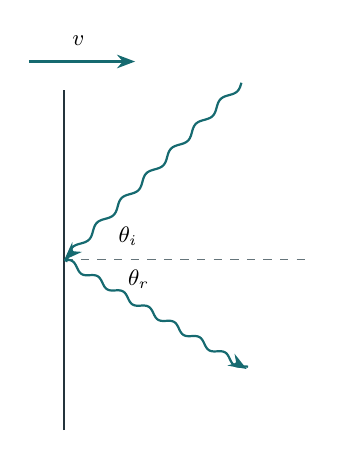
\begin{tikzpicture}[scale=.9,transform shape]
\draw[object] (0.00000,-2.40000)--(0.00000,2.40000);\draw[guide] (0.00000,0.00000)--(3.50000,0.00000);\draw[traj] plot coordinates {(2.50000,2.50000) (2.49214,2.47189) (2.48322,2.44484) (2.47231,2.41977) (2.45867,2.39744) (2.44186,2.37829) (2.42173,2.36244) (2.39853,2.34967) (2.37279,2.33944) (2.34532,2.33094) (2.31710,2.32319) (2.28920,2.31512) (2.26264,2.30571) (2.23832,2.29405) (2.21690,2.27951) (2.19872,2.26171) (2.18382,2.24064) (2.17188,2.21661) (2.16225,2.19027) (2.15408,2.16246) (2.14635,2.13423) (2.13798,2.10662) (2.12799,2.08064) (2.11554,2.05712) (2.10005,2.03664) (2.08127,2.01945) (2.05928,2.00547) (2.03449,1.99429) (2.00761,1.98519) (1.97957,1.97726) (1.95141,1.96945) (1.92419,1.96071) (1.89886,1.95006) (1.87619,1.93676) (1.85667,1.92031) (1.84046,1.90055) (1.82736,1.87767) (1.81688,1.85218) (1.80824,1.82486) (1.80045,1.79667) (1.79247,1.76868) (1.78326,1.74192) (1.77190,1.71731) (1.75770,1.69554) (1.74027,1.67700) (1.71955,1.66174) (1.69584,1.64949) (1.66971,1.63964) (1.64202,1.63136) (1.61378,1.62363) (1.58605,1.61539) (1.55985,1.60562) (1.53602,1.59348) (1.51517,1.57835) (1.49761,1.55994) (1.48329,1.53829) (1.47182,1.51379) (1.46254,1.48710) (1.45453,1.45914) (1.44676,1.43094) (1.43817,1.40356) (1.42778,1.37798) (1.41480,1.35498) (1.39872,1.33510) (1.37933,1.31851) (1.35678,1.30509) (1.33155,1.29435) (1.30438,1.28555) (1.27624,1.27772) (1.24817,1.26981) (1.22123,1.26078) (1.19634,1.24970) (1.17423,1.23585) (1.15531,1.21879) (1.13969,1.19844) (1.12713,1.17503) (1.11705,1.14914) (1.10864,1.12158) (1.10090,1.09334) (1.09277,1.06550) (1.08322,1.03908) (1.07138,1.01495) (1.05661,0.99375) (1.03857,0.97582) (1.01727,0.96114) (0.99306,0.94939) (0.96658,0.93990) (0.93871,0.93179) (0.91048,0.92405) (0.88296,0.91560) (0.85713,0.90546) (0.83382,0.89280) (0.81356,0.87708) (0.79661,0.85807) (0.78285,0.83585) (0.77184,0.81089) (0.76287,0.78390) (0.75498,0.75581) (0.74714,0.72768) (0.73828,0.70056) (0.72747,0.67541) (0.71395,0.65295) (0.69727,0.63367) (0.67728,0.61769) (0.65419,0.60480) (0.62854,0.59448) (0.60112,0.58593) (0.57291,0.57817) (0.54497,0.57014) (0.51834,0.56079) (0.49392,0.54925) (0.47237,0.53483) (0.45406,0.51716) (0.43904,0.49622) (0.42698,0.47230) (0.41728,0.44603) (0.40907,0.41827) (0.40134,0.39003) (0.39302,0.36238) (0.38311,0.33632) (0.37077,0.31269) (0.35541,0.29207) (0.33676,0.27475) (0.31489,0.26065) (0.29021,0.24936) (0.26340,0.24020) (0.23538,0.23224) (0.20721,0.22445) (0.17992,0.21576) (0.15450,0.20521) (0.13172,0.19202) (0.11207,0.17570) (0.09572,0.15608) (0.08251,0.13332) (0.07193,0.10792) (0.06323,0.08065) (0.05544,0.05248) (0.04748,0.02446) (0.03834,-0.00237) (0.02708,-0.02708)};\draw[motion] (0.12728,0.12728)--(0.00000,0.00000);\draw[traj] plot coordinates {(0.00000,0.00000) (0.02587,0.00121) (0.05098,0.00115) (0.07464,-0.00134) (0.09632,-0.00714) (0.11569,-0.01680) (0.13266,-0.03047) (0.14740,-0.04787) (0.16030,-0.06836) (0.17194,-0.09095) (0.18303,-0.11445) (0.19436,-0.13756) (0.20667,-0.15904) (0.22059,-0.17780) (0.23662,-0.19305) (0.25501,-0.20435) (0.27578,-0.21168) (0.29868,-0.21543) (0.32327,-0.21636) (0.34892,-0.21552) (0.37489,-0.21415) (0.40039,-0.21354) (0.42472,-0.21492) (0.44726,-0.21928) (0.46760,-0.22732) (0.48554,-0.23936) (0.50116,-0.25530) (0.51475,-0.27463) (0.52682,-0.29650) (0.53804,-0.31978) (0.54918,-0.34321) (0.56100,-0.36550) (0.57420,-0.38548) (0.58933,-0.40224) (0.60674,-0.41518) (0.62655,-0.42411) (0.64862,-0.42924) (0.67259,-0.43121) (0.69790,-0.43095) (0.72382,-0.42964) (0.74961,-0.42857) (0.77450,-0.42900) (0.79783,-0.43203) (0.81910,-0.43851) (0.83803,-0.44891) (0.85458,-0.46330) (0.86894,-0.48133) (0.88156,-0.50229) (0.89304,-0.52514) (0.90412,-0.54866) (0.91557,-0.57157) (0.92813,-0.59262) (0.94242,-0.61079) (0.95887,-0.62533) (0.97770,-0.63589) (0.99888,-0.64252) (1.02214,-0.64568) (1.04698,-0.64620) (1.07274,-0.64517) (1.09868,-0.64384) (1.12402,-0.64351) (1.14806,-0.64537) (1.17022,-0.65036) (1.19012,-0.65913) (1.20763,-0.67191) (1.22284,-0.68852) (1.23611,-0.70839) (1.24797,-0.73061) (1.25912,-0.75402) (1.27033,-0.77733) (1.28235,-0.79928) (1.29587,-0.81873) (1.31140,-0.83482) (1.32925,-0.84702) (1.34949,-0.85522) (1.37195,-0.85972) (1.39621,-0.86119) (1.42168,-0.86065) (1.44764,-0.85928) (1.47332,-0.85840) (1.49797,-0.85923) (1.52095,-0.86285) (1.54181,-0.87002) (1.56029,-0.88116) (1.57642,-0.89626) (1.59042,-0.91489) (1.60278,-0.93628) (1.61413,-0.95935) (1.62522,-0.98286) (1.63682,-1.00551) (1.64966,-1.02610) (1.66431,-1.04365) (1.68119,-1.05748) (1.70047,-1.06730) (1.72206,-1.07324) (1.74565,-1.07585) (1.77071,-1.07599) (1.79656,-1.07481) (1.82245,-1.07357) (1.84760,-1.07356) (1.87133,-1.07593) (1.89310,-1.08158) (1.91256,-1.09108) (1.92963,-1.10459) (1.94446,-1.12185) (1.95742,-1.14223) (1.96910,-1.16476) (1.98020,-1.18825) (1.99150,-1.21140) (2.00375,-1.23297) (2.01761,-1.25186) (2.03354,-1.26726) (2.05184,-1.27872) (2.07251,-1.28621) (2.09533,-1.29009) (2.11987,-1.29111) (2.14549,-1.29032) (2.17145,-1.28895) (2.19699,-1.28829) (2.22138,-1.28956) (2.24400,-1.29378) (2.26443,-1.30167) (2.28248,-1.31355) (2.29818,-1.32934) (2.31184,-1.34855) (2.32396,-1.37033) (2.33521,-1.39358) (2.34634,-1.41703) (2.35812,-1.43938) (2.37125,-1.45948) (2.38629,-1.47638) (2.40360,-1.48948) (2.42332,-1.49857) (2.44530,-1.50385) (2.46921,-1.50593) (2.49447,-1.50573) (2.52039,-1.50444) (2.54620,-1.50334) (2.57113,-1.50368) (2.59454,-1.50660)};\draw[motion] (2.42040,-1.44710)--(2.57489,-1.53946);\node[above] at (0.90000,0.08000) {$\theta_i$};\node[below] at (1.05000,-0.02000) {$\theta_r$};\draw[motion] (-0.50000,2.80000)--(1.00000,2.80000);\node[above] at (0.20000,2.90000) {$v$};
\end{tikzpicture}
\figcaption{图近2.4\quad 入射从右侧来，两个角从各自规定法线量起。}
\end{minipage}\end{center}

\workarea

\clearpage

\pdfbookmark[2]{第 5 题 共同运动的介质界面}{q5}

\section*{第 5 题\quad 共同运动的介质界面}\label{q:5}

两种均匀、透明、各向同性且无色散的介质与它们的平面界面共同以$v=\beta c$沿实验室系$S$的$+x$运动，$0\le\beta<1$，界面法线为$x$轴。两介质在共同静止系$S'$的折射率为$n_1,n_2\ge1$。光从介质1射向介质2；在$S$中，入射角$\theta_i$从$+x$量起，反射角$\theta_r$从$-x$量起，折射角$\theta_t$从$+x$量起，均取图示正横向分量。

求实验室中反射角、折射角与入射角的关系，说明传播分支与适用角域；再给出介质1为真空、介质2折射率为$n$时的结果。只讨论能射到界面的入射支；若发生全反射，应指出没有传播折射光。

\begin{center}\begin{minipage}{.98\linewidth}\centering
\begin{tikzpicture}[scale=.9,transform shape]
\draw[object] (0.00000,-2.80000)--(0.00000,2.80000);\draw[guide] (-3.20000,0.00000)--(3.80000,0.00000);\draw[traj] plot coordinates {(-2.38415,-1.82094) (-2.37569,-1.79646) (-2.36632,-1.77317) (-2.35524,-1.75212) (-2.34182,-1.73413) (-2.32567,-1.71972) (-2.30669,-1.70902) (-2.28506,-1.70178) (-2.26125,-1.69740) (-2.23595,-1.69496) (-2.21002,-1.69336) (-2.18435,-1.69141) (-2.15984,-1.68794) (-2.13725,-1.68196) (-2.11715,-1.67272) (-2.09984,-1.65983) (-2.08533,-1.64326) (-2.07336,-1.62338) (-2.06339,-1.60088) (-2.05466,-1.57675) (-2.04631,-1.55212) (-2.03742,-1.52821) (-2.02713,-1.50613) (-2.01472,-1.48681) (-1.99972,-1.47090) (-1.98188,-1.45869) (-1.96129,-1.45010) (-1.93830,-1.44464) (-1.91351,-1.44153) (-1.88773,-1.43973) (-1.86184,-1.43807) (-1.83676,-1.43535) (-1.81331,-1.43050) (-1.79213,-1.42267) (-1.77366,-1.41129) (-1.75803,-1.39620) (-1.74508,-1.37760) (-1.73437,-1.35607) (-1.72524,-1.33247) (-1.71684,-1.30790) (-1.70828,-1.28356) (-1.69865,-1.26060) (-1.68719,-1.24006) (-1.67329,-1.22270) (-1.65661,-1.20897) (-1.63712,-1.19894) (-1.61504,-1.19228) (-1.59091,-1.18833) (-1.56542,-1.18613) (-1.53947,-1.18456) (-1.51395,-1.18241) (-1.48974,-1.17855) (-1.46758,-1.17202) (-1.44797,-1.16213) (-1.43118,-1.14855) (-1.41717,-1.13133) (-1.40562,-1.11091) (-1.39593,-1.08803) (-1.38734,-1.06372) (-1.37896,-1.03914) (-1.36987,-1.01548) (-1.35924,-0.99384) (-1.34639,-0.97511) (-1.33087,-0.95987) (-1.31251,-0.94835) (-1.29145,-0.94037) (-1.26807,-0.93542) (-1.24304,-0.93264) (-1.21717,-0.93095) (-1.19136,-0.92918) (-1.16652,-0.92615) (-1.14345,-0.92081) (-1.12275,-0.91235) (-1.10480,-0.90029) (-1.08968,-0.88453) (-1.07718,-0.86534) (-1.06682,-0.84335) (-1.05788,-0.81949) (-1.04953,-0.79487) (-1.04083,-0.77069) (-1.03092,-0.74811) (-1.01905,-0.72810) (-1.00465,-0.71139) (-0.98746,-0.69835) (-0.96746,-0.68897) (-0.94496,-0.68287) (-0.92052,-0.67932) (-0.89488,-0.67733) (-0.86894,-0.67574) (-0.84360,-0.67336) (-0.81971,-0.66907) (-0.79799,-0.66196) (-0.77889,-0.65141) (-0.76262,-0.63715) (-0.74910,-0.61930) (-0.73794,-0.59835) (-0.72852,-0.57513) (-0.72003,-0.55068) (-0.71159,-0.52618) (-0.70228,-0.50281) (-0.69128,-0.48165) (-0.67796,-0.46353) (-0.66193,-0.44897) (-0.64305,-0.43812) (-0.62152,-0.43076) (-0.59779,-0.42627) (-0.57254,-0.42378) (-0.54661,-0.42217) (-0.52092,-0.42025) (-0.49634,-0.41686) (-0.47367,-0.41100) (-0.45345,-0.40191) (-0.43603,-0.38917) (-0.42141,-0.37274) (-0.40935,-0.35298) (-0.39931,-0.33057) (-0.39055,-0.30648) (-0.38220,-0.28185) (-0.37335,-0.25789) (-0.36313,-0.23571) (-0.35082,-0.21627) (-0.33592,-0.20021) (-0.31820,-0.18786) (-0.29772,-0.17912) (-0.27481,-0.17355) (-0.25009,-0.17037) (-0.22433,-0.16854) (-0.19842,-0.16689) (-0.17329,-0.16424) (-0.14976,-0.15950) (-0.12849,-0.15179) (-0.10990,-0.14056) (-0.09416,-0.12562) (-0.08110,-0.10716) (-0.07032,-0.08572) (-0.06113,-0.06219) (-0.05273,-0.03764) (-0.04419,-0.01326) (-0.03462,0.00977) (-0.02324,0.03043)};\draw[motion] (-0.14305,-0.10926)--(0.00000,0.00000);\draw[traj] plot coordinates {(0.00000,0.00000) (-0.02430,0.00896) (-0.04740,0.01880) (-0.06822,0.03031) (-0.08593,0.04409) (-0.10001,0.06053) (-0.11032,0.07973) (-0.11711,0.10150) (-0.12101,0.12540) (-0.12293,0.15074) (-0.12400,0.17670) (-0.12543,0.20240) (-0.12840,0.22698) (-0.13392,0.24968) (-0.14274,0.26997) (-0.15528,0.28754) (-0.17154,0.30238) (-0.19118,0.31476) (-0.21347,0.32519) (-0.23742,0.33440) (-0.26187,0.34326) (-0.28559,0.35264) (-0.30746,0.36337) (-0.32653,0.37617) (-0.34212,0.39150) (-0.35396,0.40958) (-0.36214,0.43034) (-0.36712,0.45344) (-0.36972,0.47828) (-0.37100,0.50410) (-0.37213,0.53001) (-0.37434,0.55515) (-0.37871,0.57869) (-0.38611,0.60002) (-0.39711,0.61872) (-0.41187,0.63466) (-0.43020,0.64799) (-0.45152,0.65913) (-0.47492,0.66875) (-0.49931,0.67764) (-0.52348,0.68670) (-0.54624,0.69679) (-0.56654,0.70867) (-0.58361,0.72293) (-0.59699,0.73988) (-0.60663,0.75957) (-0.61283,0.78178) (-0.61629,0.80599) (-0.61797,0.83151) (-0.61901,0.85749) (-0.62064,0.88305) (-0.62400,0.90733) (-0.63008,0.92963) (-0.63957,0.94943) (-0.65280,0.96649) (-0.66973,0.98085) (-0.68992,0.99282) (-0.71259,1.00297) (-0.73672,1.01205) (-0.76113,1.02094) (-0.78460,1.03050) (-0.80601,1.04158) (-0.82448,1.05481) (-0.83940,1.07063) (-0.85054,1.08922) (-0.85808,1.11045) (-0.86256,1.13392) (-0.86483,1.15900) (-0.86599,1.18490) (-0.86723,1.21074) (-0.86976,1.23564) (-0.87463,1.25882) (-0.88266,1.27968) (-0.89435,1.29788) (-0.90980,1.31331) (-0.92873,1.32620) (-0.95050,1.33701) (-0.97418,1.34643) (-0.99862,1.35529) (-1.02261,1.36447) (-1.04499,1.37484) (-1.06475,1.38712) (-1.08116,1.40185) (-1.09385,1.41931) (-1.10282,1.43950) (-1.10846,1.46212) (-1.11151,1.48663) (-1.11298,1.51230) (-1.11404,1.53827) (-1.11590,1.56365) (-1.11970,1.58762) (-1.12637,1.60949) (-1.13653,1.62880) (-1.15045,1.64535) (-1.16802,1.65924) (-1.18874,1.67082) (-1.21176,1.68071) (-1.23604,1.68969) (-1.26036,1.69864) (-1.28353,1.70842) (-1.30446,1.71985) (-1.32231,1.73353) (-1.33654,1.74986) (-1.34700,1.76895) (-1.35392,1.79063) (-1.35792,1.81445) (-1.35990,1.83975) (-1.36098,1.86570) (-1.36237,1.89143) (-1.36526,1.91607) (-1.37066,1.93886) (-1.37934,1.95925) (-1.39172,1.97694) (-1.40784,1.99188) (-1.42736,2.00435) (-1.44956,2.01484) (-1.47346,2.02409) (-1.49791,2.03294) (-1.52169,2.04228) (-1.54365,2.05295) (-1.56284,2.06566) (-1.57859,2.08088) (-1.59058,2.09885) (-1.59890,2.11951) (-1.60400,2.14252) (-1.60668,2.16731) (-1.60798,2.19310) (-1.60910,2.21903) (-1.61124,2.24421) (-1.61550,2.26783) (-1.62277,2.28926) (-1.63361,2.30807) (-1.64823,2.32411) (-1.66643,2.33754) (-1.68763,2.34877) (-1.71098,2.35843) (-1.73535,2.36733) (-1.75955,2.37637) (-1.78238,2.38640) (-1.80280,2.39820)};\draw[motion] (-1.66559,2.27557)--(-1.77191,2.42082);\draw[traj] plot coordinates {(0.00000,0.00000) (0.01489,0.02119) (0.03032,0.04099) (0.04678,0.05817) (0.06465,0.07175) (0.08415,0.08114) (0.10535,0.08619) (0.12814,0.08717) (0.15223,0.08481) (0.17722,0.08017) (0.20259,0.07455) (0.22780,0.06934) (0.25231,0.06591) (0.27567,0.06542) (0.29755,0.06874) (0.31774,0.07636) (0.33626,0.08828) (0.35325,0.10408) (0.36905,0.12295) (0.38410,0.14374) (0.39893,0.16510) (0.41408,0.18563) (0.43006,0.20401) (0.44732,0.21916) (0.46613,0.23030) (0.48665,0.23711) (0.50881,0.23969) (0.53241,0.23858) (0.55709,0.23473) (0.58237,0.22934) (0.60771,0.22379) (0.63257,0.21948) (0.65645,0.21766) (0.67896,0.21935) (0.69986,0.22519) (0.71905,0.23537) (0.73663,0.24967) (0.75287,0.26742) (0.76816,0.28757) (0.78301,0.30887) (0.79797,0.32990) (0.81355,0.34931) (0.83025,0.36589) (0.84840,0.37873) (0.86822,0.38732) (0.88972,0.39159) (0.91278,0.39189) (0.93707,0.38902) (0.96216,0.38410) (0.98755,0.37845) (1.01266,0.37347) (1.03700,0.37049) (1.06011,0.37065) (1.08168,0.37475) (1.10157,0.38316) (1.11978,0.39584) (1.13653,0.41228) (1.15215,0.43160) (1.16712,0.45259) (1.18196,0.47391) (1.19723,0.49414) (1.21342,0.51200) (1.23095,0.52645) (1.25007,0.53681) (1.27089,0.54282) (1.29334,0.54467) (1.31718,0.54298) (1.34200,0.53874) (1.36734,0.53322) (1.39263,0.52779) (1.41734,0.52385) (1.44100,0.52262) (1.46322,0.52503) (1.48380,0.53166) (1.50269,0.54264) (1.52000,0.55763) (1.53603,0.57591) (1.55120,0.59637) (1.56603,0.61773) (1.58106,0.63856) (1.59682,0.65753) (1.61376,0.67348) (1.63221,0.68557) (1.65234,0.69336) (1.67414,0.69685) (1.69745,0.69650) (1.72193,0.69317) (1.74712,0.68800) (1.77249,0.68237) (1.79750,0.67766) (1.82164,0.67519) (1.84449,0.67602) (1.86576,0.68089) (1.88533,0.69011) (1.90326,0.70353) (1.91977,0.72058) (1.93523,0.74030) (1.95013,0.76146) (1.96502,0.78268) (1.98042,0.80256) (1.99683,0.81987) (2.01463,0.83361) (2.03406,0.84317) (2.05520,0.84839) (2.07793,0.84953) (2.10197,0.84728) (2.12693,0.84271) (2.15230,0.83710) (2.17752,0.83185) (2.20207,0.82832) (2.22549,0.82769) (2.24743,0.83085) (2.26769,0.83829) (2.28627,0.85004) (2.30333,0.86570) (2.31916,0.88447) (2.33423,0.90520) (2.34906,0.92657) (2.36418,0.94716) (2.38013,0.96565) (2.39732,0.98094) (2.41607,0.99226) (2.43652,0.99924) (2.45862,1.00198) (2.48217,1.00101) (2.50681,0.99725) (2.53208,0.99189) (2.55743,0.98632) (2.58231,0.98193) (2.60624,0.98000) (2.62882,0.98153) (2.64978,0.98719) (2.66904,0.99720) (2.68668,1.01135) (2.70297,1.02897) (2.71829,1.04905) (2.73315,1.07033) (2.74809,1.09140) (2.76364,1.11090) (2.78028,1.12761)};\draw[motion] (2.62656,1.02643)--(2.79422,1.09195);\node[above] at (-2.00000,2.80000) {介质1};\node[above] at (2.00000,2.80000) {介质2};\node[below] at (-1.10000,-0.04000) {$\theta_i$};\node[above] at (-1.05000,0.06000) {$\theta_r$};\node[below] at (1.65000,-0.04000) {$\theta_t$};\draw[motion] (-0.50000,3.50000)--(1.00000,3.50000);\node[above] at (0.25000,3.60000) {$v$};
\end{tikzpicture}
\figcaption{图近2.5\quad 界面和两介质共同移动，三角均按传播方向定义。}
\end{minipage}\end{center}

\workarea

\clearpage

\pdfbookmark[2]{第 6 题 运动观察者所见的星空分布}{q6}

\section*{第 6 题\quad 运动观察者所见的星空分布}\label{q:6}

惯性系$S'$相对$S$以$v=\beta c$沿$+z$运动，$0\le\beta<1$。两观察点之间的距离远小于它们至恒星的距离，忽略视差。$S$的观察者看到的恒星数在天空上各向同性，每单位立体角有$N$颗；假定所有恒星均可计数，不设流量阈值。

取指向恒星的方向与$+z$的夹角为$\theta$，在$S'$中对应角为$\theta'$。求$S'$所见的每单位立体角星数$N'(\theta',\phi')$，并讨论高速极限。

\begin{center}\begin{minipage}{.98\linewidth}\centering
\begin{tikzpicture}[scale=.9,transform shape]
\draw[object] (0.00000,0.00000) circle(2.00000);\draw[axis] (0.00000,0.00000)--(2.80000,0.00000);\node[below right] at (2.80000,0.00000) {$+z$};\fill (0.00000,0.00000) circle(.035);\node[below] at (0.00000,0.00000) {观察者};\fill (1.81262,0.84524) circle(.035);\draw[guide] (0.00000,0.00000)--(1.81262,0.84524);\fill (1.28558,1.53209) circle(.035);\draw[guide] (0.00000,0.00000)--(1.28558,1.53209);\fill (0.51764,1.93185) circle(.035);\draw[guide] (0.00000,0.00000)--(0.51764,1.93185);\fill (-0.34730,1.96962) circle(.035);\draw[guide] (0.00000,0.00000)--(-0.34730,1.96962);\fill (-1.14715,1.63830) circle(.035);\draw[guide] (0.00000,0.00000)--(-1.14715,1.63830);\fill (-1.73205,1.00000) circle(.035);\draw[guide] (0.00000,0.00000)--(-1.73205,1.00000);\fill (1.81262,-0.84524) circle(.035);\draw[guide] (0.00000,0.00000)--(1.81262,-0.84524);\fill (1.28558,-1.53209) circle(.035);\draw[guide] (0.00000,0.00000)--(1.28558,-1.53209);\fill (0.51764,-1.93185) circle(.035);\draw[guide] (0.00000,0.00000)--(0.51764,-1.93185);\fill (-0.34730,-1.96962) circle(.035);\draw[guide] (0.00000,0.00000)--(-0.34730,-1.96962);\fill (-1.14715,-1.63830) circle(.035);\draw[guide] (0.00000,0.00000)--(-1.14715,-1.63830);\fill (-1.73205,-1.00000) circle(.035);\draw[guide] (0.00000,0.00000)--(-1.73205,-1.00000);\node[above] at (0.00000,2.80000) {$S$中星空的子午截面};\node[below] at (0.00000,-2.80000) {方向从观察者指向恒星};
\end{tikzpicture}
\figcaption{图近2.6\quad 忽略视差与亮度选样，只研究恒星方位的变换。}
\end{minipage}\end{center}

\workarea

\clearpage

\pdfbookmark[2]{第 7 题 运动点光源的接收强度}{q7}

\section*{第 7 题\quad 运动点光源的接收强度}\label{q:7}

单色点光源在自身静止系$S'$向各方向均匀辐射，每单位本征时间、每单位立体角的辐射能为$I_0$。光源在实验室系$S$中以$v=\beta c$沿$+x$运动。远处固定探测器接收光源发出的光，$\theta$为发射点至探测器的光传播方向与$+x$的夹角；考察短时间内方向近似不变的情况。

将几何距离平方衰减因素除去，定义$I_{\rm rec}=\dd E/(\dd t_{\rm arr}\dd\Omega)$，其中$t_{\rm arr}$为探测器接收时间。求$I_{\rm rec}(\theta)$，并与按实验室发射时刻定义的$I_{\rm em}=\dd E/(\dd t_{\rm em}\dd\Omega)$区分。

\begin{center}\begin{minipage}{.98\linewidth}\centering
\begin{tikzpicture}[scale=.9,transform shape]
\fill (0.00000,0.00000) circle(.035);\node[below] at (0.00000,0.00000) {光源};\draw[motion] (0.00000,1.10000)--(1.60000,1.10000);\node[above] at (0.80000,1.20000) {$v$};\draw[traj] plot coordinates {(0.00000,0.00000) (0.03864,0.02797) (0.07775,0.05453) (0.11775,0.07841) (0.15897,0.09863) (0.20161,0.11458) (0.24573,0.12611) (0.29123,0.13350) (0.33787,0.13748) (0.38527,0.13914) (0.43302,0.13980) (0.48062,0.14088) (0.52762,0.14377) (0.57361,0.14966) (0.61832,0.15944) (0.66157,0.17358) (0.70335,0.19211) (0.74382,0.21459) (0.78324,0.24020) (0.82202,0.26776) (0.86060,0.29590) (0.89946,0.32320) (0.93905,0.34831) (0.97974,0.37012) (1.02179,0.38786) (1.06531,0.40118) (1.11027,0.41020) (1.15648,0.41546) (1.20362,0.41792) (1.25128,0.41882) (1.29900,0.41955) (1.34630,0.42155) (1.39274,0.42608) (1.43800,0.43419) (1.48186,0.44652) (1.52423,0.46328) (1.56521,0.48424) (1.60502,0.50870) (1.64400,0.53561) (1.68261,0.56369) (1.72130,0.59150) (1.76054,0.61766) (1.80074,0.64093) (1.84222,0.66040) (1.88513,0.67554) (1.92952,0.68627) (1.97525,0.69296) (2.02205,0.69643) (2.06956,0.69780) (2.11731,0.69843) (2.16483,0.69975) (2.21168,0.70310) (2.25745,0.70965) (2.30190,0.72021) (2.34487,0.73517) (2.38640,0.75447) (2.42665,0.77760) (2.46592,0.80366) (2.50463,0.83144) (2.54323,0.85953) (2.58219,0.88652) (2.62196,0.91110) (2.66288,0.93221) (2.70520,0.94915) (2.74899,0.96166) (2.79420,0.96993) (2.84060,0.97459) (2.88787,0.97667) (2.93558,0.97743) (2.98326,0.97829) (3.03043,0.98066) (3.07668,0.98579) (3.12169,0.99464) (3.16527,1.00778) (3.20738,1.02534) (3.24812,1.04700) (3.28775,1.07200) (3.32663,1.09924) (3.36522,1.12737) (3.40397,1.15498) (3.44337,1.18069) (3.48378,1.20332) (3.52551,1.22202) (3.56870,1.23634) (3.61335,1.24629) (3.65930,1.25232) (3.70626,1.25531) (3.75385,1.25644) (3.80160,1.25708) (3.84903,1.25868) (3.89570,1.26255) (3.94125,1.26978) (3.98543,1.28113) (4.02813,1.29690) (4.06941,1.31696) (4.10945,1.34071) (4.14859,1.36719) (4.18724,1.39513) (4.22587,1.42312) (4.26495,1.44976) (4.30490,1.47378) (4.34607,1.49416) (4.38866,1.51029) (4.43272,1.52199) (4.47816,1.52954) (4.52476,1.53364) (4.57214,1.53537) (4.61988,1.53604) (4.66750,1.53708) (4.71453,1.53987) (4.76057,1.54562) (4.80533,1.55522) (4.84864,1.56918) (4.89048,1.58754) (4.93100,1.60988) (4.97046,1.63538) (5.00925,1.66289) (5.04783,1.69104) (5.08667,1.71840) (5.12623,1.74362) (5.16687,1.76558) (5.20886,1.78350) (5.25232,1.79700) (5.29722,1.80617) (5.34339,1.81157) (5.39050,1.81412) (5.43815,1.81506) (5.48587,1.81577) (5.53319,1.81769) (5.57968,1.82210) (5.62500,1.83005) (5.66891,1.84220) (5.71134,1.85879) (5.75237,1.87958) (5.79222,1.90392) (5.83123,1.93076) (5.86984,1.95882) (5.90852,1.98667) (5.94773,2.01292) (5.98789,2.03633)};\draw[motion] (5.82924,1.94308)--(6.00000,2.00000);\fill (6.00000,2.00000) circle(.035);\node[above right] at (6.00000,2.00000) {探测器 $P$};\draw[guide] (0.00000,0.00000)--(6.00000,0.00000);\node[below] at (1.60000,-0.10000) {$\theta$};\draw[guide] plot coordinates {(0.80000,0.00000) (0.79989,0.01355) (0.79954,0.02709) (0.79897,0.04062) (0.79817,0.05415) (0.79713,0.06766) (0.79587,0.08114) (0.79439,0.09461) (0.79267,0.10805) (0.79073,0.12146) (0.78856,0.13483) (0.78616,0.14816) (0.78354,0.16145) (0.78069,0.17470) (0.77762,0.18789) (0.77433,0.20103) (0.77081,0.21412) (0.76708,0.22714) (0.76312,0.24009) (0.75895,0.25298)};
\end{tikzpicture}
\figcaption{图近2.7\quad 角度沿发射点至接收器的光传播方向。}
\end{minipage}\end{center}

\workarea

\clearpage

\pdfbookmark[2]{第 8 题 迎面反射镜返回的光功率}{q8}

\section*{第 8 题\quad 迎面反射镜返回的光功率}\label{q:8}

固定光源在实验室系$S$中发出一束平行光，功率为$P_0$。理想平面镜垂直光束，并以恒定速率$v=\beta c$朝光源运动，$0<\beta<1$。镜面截获全部光束，反射光全部返回光源处的固定探测器。求探测器按接收时间测得的反射光功率，说明能量交换。镜速由外部机构维持，忽略镜面反冲对其速度的改变。

\begin{center}\begin{minipage}{.98\linewidth}\centering
\begin{tikzpicture}[scale=.9,transform shape]
\fill (0.00000,0.00000) circle(.035);\node[below] at (0.00000,0.00000) {定源与探测器};\draw[object] (6.00000,-1.60000)--(6.00000,2.20000);\draw[traj] plot coordinates {(0.00000,0.50000) (0.04317,0.51432) (0.08633,0.52714) (0.12950,0.53715) (0.17266,0.54330) (0.21583,0.54495) (0.25899,0.54193) (0.30216,0.53455) (0.34532,0.52358) (0.38849,0.51017) (0.43165,0.49569) (0.47482,0.48167) (0.51799,0.46955) (0.56115,0.46059) (0.60432,0.45573) (0.64748,0.45546) (0.69065,0.45983) (0.73381,0.46837) (0.77698,0.48019) (0.82014,0.49407) (0.86331,0.50857) (0.90647,0.52218) (0.94964,0.53348) (0.99281,0.54131) (1.03597,0.54484) (1.07914,0.54372) (1.12230,0.53805) (1.16547,0.52843) (1.20863,0.51585) (1.25180,0.50163) (1.29496,0.48724) (1.33813,0.47418) (1.38129,0.46379) (1.42446,0.45717) (1.46763,0.45500) (1.51079,0.45751) (1.55396,0.46443) (1.59712,0.47504) (1.64029,0.48825) (1.68345,0.50268) (1.72662,0.51683) (1.76978,0.52923) (1.81295,0.53860) (1.85612,0.54395) (1.89928,0.54474) (1.94245,0.54088) (1.98561,0.53277) (2.02878,0.52126) (2.07194,0.50754) (2.11511,0.49304) (2.15827,0.47926) (2.20144,0.46763) (2.24460,0.45937) (2.28777,0.45533) (2.33094,0.45593) (2.37410,0.46111) (2.41727,0.47033) (2.46043,0.48263) (2.50360,0.49674) (2.54676,0.51118) (2.58993,0.52447) (2.63309,0.53521) (2.67626,0.54230) (2.71942,0.54499) (2.76259,0.54300) (2.80576,0.53655) (2.84892,0.52630) (2.89209,0.51332) (2.93525,0.49895) (2.97842,0.48470) (3.02158,0.47203) (3.06475,0.46227) (3.10791,0.45643) (3.15108,0.45511) (3.19424,0.45846) (3.23741,0.46613) (3.28058,0.47731) (3.32374,0.49085) (3.36691,0.50534) (3.41007,0.51928) (3.45324,0.53121) (3.49640,0.53990) (3.53957,0.54445) (3.58273,0.54437) (3.62590,0.53969) (3.66906,0.53088) (3.71223,0.51887) (3.75540,0.50489) (3.79856,0.49040) (3.84173,0.47692) (3.88489,0.46583) (3.92806,0.45829) (3.97122,0.45508) (4.01439,0.45654) (4.05755,0.46252) (4.10072,0.47239) (4.14388,0.48513) (4.18705,0.49941) (4.23022,0.51376) (4.27338,0.52667) (4.31655,0.53682) (4.35971,0.54314) (4.40288,0.54497) (4.44604,0.54214) (4.48921,0.53492) (4.53237,0.52408) (4.57554,0.51074) (4.61871,0.49628) (4.66187,0.48221) (4.70504,0.46998) (4.74820,0.46088) (4.79137,0.45584) (4.83453,0.45538) (4.87770,0.45957) (4.92086,0.46795) (4.96403,0.47966) (5.00719,0.49349) (5.05036,0.50799) (5.09353,0.52167) (5.13669,0.53309) (5.17986,0.54107) (5.22302,0.54479) (5.26619,0.54385) (5.30935,0.53836) (5.35252,0.52888) (5.39568,0.51640) (5.43885,0.50222) (5.48201,0.48781) (5.52518,0.47466) (5.56835,0.46415) (5.61151,0.45736) (5.65468,0.45500) (5.69784,0.45732) (5.74101,0.46407) (5.78417,0.47455) (5.82734,0.48768) (5.87050,0.50209) (5.91367,0.51628) (5.95683,0.52878) (6.00000,0.53829)};\draw[motion] (5.82000,0.50000)--(6.00000,0.50000);\node[above] at (3.00000,0.50000) {$P_0$};\draw[traj] plot coordinates {(6.00000,-0.60000) (5.95683,-0.61432) (5.91367,-0.62714) (5.87050,-0.63715) (5.82734,-0.64330) (5.78417,-0.64495) (5.74101,-0.64193) (5.69784,-0.63455) (5.65468,-0.62358) (5.61151,-0.61017) (5.56835,-0.59569) (5.52518,-0.58167) (5.48201,-0.56955) (5.43885,-0.56059) (5.39568,-0.55573) (5.35252,-0.55546) (5.30935,-0.55983) (5.26619,-0.56837) (5.22302,-0.58019) (5.17986,-0.59407) (5.13669,-0.60857) (5.09353,-0.62218) (5.05036,-0.63348) (5.00719,-0.64131) (4.96403,-0.64484) (4.92086,-0.64372) (4.87770,-0.63805) (4.83453,-0.62843) (4.79137,-0.61585) (4.74820,-0.60163) (4.70504,-0.58724) (4.66187,-0.57418) (4.61871,-0.56379) (4.57554,-0.55717) (4.53237,-0.55500) (4.48921,-0.55751) (4.44604,-0.56443) (4.40288,-0.57504) (4.35971,-0.58825) (4.31655,-0.60268) (4.27338,-0.61683) (4.23022,-0.62923) (4.18705,-0.63860) (4.14388,-0.64395) (4.10072,-0.64474) (4.05755,-0.64088) (4.01439,-0.63277) (3.97122,-0.62126) (3.92806,-0.60754) (3.88489,-0.59304) (3.84173,-0.57926) (3.79856,-0.56763) (3.75540,-0.55937) (3.71223,-0.55533) (3.66906,-0.55593) (3.62590,-0.56111) (3.58273,-0.57033) (3.53957,-0.58263) (3.49640,-0.59674) (3.45324,-0.61118) (3.41007,-0.62447) (3.36691,-0.63521) (3.32374,-0.64230) (3.28058,-0.64499) (3.23741,-0.64300) (3.19424,-0.63655) (3.15108,-0.62630) (3.10791,-0.61332) (3.06475,-0.59895) (3.02158,-0.58470) (2.97842,-0.57203) (2.93525,-0.56227) (2.89209,-0.55643) (2.84892,-0.55511) (2.80576,-0.55846) (2.76259,-0.56613) (2.71942,-0.57731) (2.67626,-0.59085) (2.63309,-0.60534) (2.58993,-0.61928) (2.54676,-0.63121) (2.50360,-0.63990) (2.46043,-0.64445) (2.41727,-0.64437) (2.37410,-0.63969) (2.33094,-0.63088) (2.28777,-0.61887) (2.24460,-0.60489) (2.20144,-0.59040) (2.15827,-0.57692) (2.11511,-0.56583) (2.07194,-0.55829) (2.02878,-0.55508) (1.98561,-0.55654) (1.94245,-0.56252) (1.89928,-0.57239) (1.85612,-0.58513) (1.81295,-0.59941) (1.76978,-0.61376) (1.72662,-0.62667) (1.68345,-0.63682) (1.64029,-0.64314) (1.59712,-0.64497) (1.55396,-0.64214) (1.51079,-0.63492) (1.46763,-0.62408) (1.42446,-0.61074) (1.38129,-0.59628) (1.33813,-0.58221) (1.29496,-0.56998) (1.25180,-0.56088) (1.20863,-0.55584) (1.16547,-0.55538) (1.12230,-0.55957) (1.07914,-0.56795) (1.03597,-0.57966) (0.99281,-0.59349) (0.94964,-0.60799) (0.90647,-0.62167) (0.86331,-0.63309) (0.82014,-0.64107) (0.77698,-0.64479) (0.73381,-0.64385) (0.69065,-0.63836) (0.64748,-0.62888) (0.60432,-0.61640) (0.56115,-0.60222) (0.51799,-0.58781) (0.47482,-0.57466) (0.43165,-0.56415) (0.38849,-0.55736) (0.34532,-0.55500) (0.30216,-0.55732) (0.25899,-0.56407) (0.21583,-0.57455) (0.17266,-0.58768) (0.12950,-0.60209) (0.08633,-0.61628) (0.04317,-0.62878) (0.00000,-0.63829)};\draw[motion] (0.18000,-0.60000)--(0.00000,-0.60000);\node[above] at (3.00000,-0.60000) {$P_{\rm det}$};\draw[motion] (6.00000,2.50000)--(4.00000,2.50000);\node[above] at (5.00000,2.60000) {朝源 $v$};
\end{tikzpicture}
\figcaption{图近2.8\quad 移动镜迎向入射平行光，反射光返回固定探测器。}
\end{minipage}\end{center}

\workarea

\clearpage

\pdfbookmark[2]{第 9 题 移动色散介质中的相速度}{q9}

\section*{第 9 题\quad 移动色散介质中的相速度}\label{q:9}

单色光源固定在实验室系$S$中，向$+x$发光。一整块透明色散介质及它的入射端面共同以$v$沿$+x$匀速移动，$|v|\ll c$，端面法线沿$x$。在介质静止时，这束光在介质内的物理波长为$\lambda$，折射率为$n=n(\lambda)$；给定以该物理波长为自变量的导数$D_\lambda=\dd n/\dd\lambda$。

在频移范围内作一阶展开，求实验室看到的介质内相速度。说明波长自变量和移动边界条件怎样进入色散修正。设$n+\lambda D_\lambda\ne0$，介质在考察频段内可用平滑实折射率描述。

\begin{center}\begin{minipage}{.98\linewidth}\centering
\begin{tikzpicture}[scale=.9,transform shape]
\draw[object] (-0.80000,-0.35000)--(0.80000,-0.35000)--(0.80000,0.35000)--(-0.80000,0.35000)--(-0.80000,-0.35000);\node[anchor=center] at (0.00000,0.00000) {定源};\draw[object] (3.00000,-1.20000)--(7.00000,-1.20000)--(7.00000,1.20000)--(3.00000,1.20000)--(3.00000,-1.20000);\draw[traj] plot coordinates {(1.00000,0.00000) (1.01439,0.01432) (1.02878,0.02714) (1.04317,0.03715) (1.05755,0.04330) (1.07194,0.04495) (1.08633,0.04193) (1.10072,0.03455) (1.11511,0.02358) (1.12950,0.01017) (1.14388,-0.00431) (1.15827,-0.01833) (1.17266,-0.03045) (1.18705,-0.03941) (1.20144,-0.04427) (1.21583,-0.04454) (1.23022,-0.04017) (1.24460,-0.03163) (1.25899,-0.01981) (1.27338,-0.00593) (1.28777,0.00857) (1.30216,0.02218) (1.31655,0.03348) (1.33094,0.04131) (1.34532,0.04484) (1.35971,0.04372) (1.37410,0.03805) (1.38849,0.02843) (1.40288,0.01585) (1.41727,0.00163) (1.43165,-0.01276) (1.44604,-0.02582) (1.46043,-0.03621) (1.47482,-0.04283) (1.48921,-0.04500) (1.50360,-0.04249) (1.51799,-0.03557) (1.53237,-0.02496) (1.54676,-0.01175) (1.56115,0.00268) (1.57554,0.01683) (1.58993,0.02923) (1.60432,0.03860) (1.61871,0.04395) (1.63309,0.04474) (1.64748,0.04088) (1.66187,0.03277) (1.67626,0.02126) (1.69065,0.00754) (1.70504,-0.00696) (1.71942,-0.02074) (1.73381,-0.03237) (1.74820,-0.04063) (1.76259,-0.04467) (1.77698,-0.04407) (1.79137,-0.03889) (1.80576,-0.02967) (1.82014,-0.01737) (1.83453,-0.00326) (1.84892,0.01118) (1.86331,0.02447) (1.87770,0.03521) (1.89209,0.04230) (1.90647,0.04499) (1.92086,0.04300) (1.93525,0.03655) (1.94964,0.02630) (1.96403,0.01332) (1.97842,-0.00105) (1.99281,-0.01530) (2.00719,-0.02797) (2.02158,-0.03773) (2.03597,-0.04357) (2.05036,-0.04489) (2.06475,-0.04154) (2.07914,-0.03387) (2.09353,-0.02269) (2.10791,-0.00915) (2.12230,0.00534) (2.13669,0.01928) (2.15108,0.03121) (2.16547,0.03990) (2.17986,0.04445) (2.19424,0.04437) (2.20863,0.03969) (2.22302,0.03088) (2.23741,0.01887) (2.25180,0.00489) (2.26619,-0.00960) (2.28058,-0.02308) (2.29496,-0.03417) (2.30935,-0.04171) (2.32374,-0.04492) (2.33813,-0.04346) (2.35252,-0.03748) (2.36691,-0.02761) (2.38129,-0.01487) (2.39568,-0.00059) (2.41007,0.01376) (2.42446,0.02667) (2.43885,0.03682) (2.45324,0.04314) (2.46763,0.04497) (2.48201,0.04214) (2.49640,0.03492) (2.51079,0.02408) (2.52518,0.01074) (2.53957,-0.00372) (2.55396,-0.01779) (2.56835,-0.03002) (2.58273,-0.03912) (2.59712,-0.04416) (2.61151,-0.04462) (2.62590,-0.04043) (2.64029,-0.03205) (2.65468,-0.02034) (2.66906,-0.00651) (2.68345,0.00799) (2.69784,0.02167) (2.71223,0.03309) (2.72662,0.04107) (2.74101,0.04479) (2.75540,0.04385) (2.76978,0.03836) (2.78417,0.02888) (2.79856,0.01640) (2.81295,0.00222) (2.82734,-0.01219) (2.84173,-0.02534) (2.85612,-0.03585) (2.87050,-0.04264) (2.88489,-0.04500) (2.89928,-0.04268) (2.91367,-0.03593) (2.92806,-0.02545) (2.94245,-0.01232) (2.95683,0.00209) (2.97122,0.01628) (2.98561,0.02878) (3.00000,0.03829)};\draw[motion] (2.82000,0.00000)--(3.00000,0.00000);\node[above] at (2.00000,0.00000) {$\Lambda$};\draw[traj] plot coordinates {(3.00000,0.00000) (3.02662,0.01432) (3.05324,0.02714) (3.07986,0.03715) (3.10647,0.04330) (3.13309,0.04495) (3.15971,0.04193) (3.18633,0.03455) (3.21295,0.02358) (3.23957,0.01017) (3.26619,-0.00431) (3.29281,-0.01833) (3.31942,-0.03045) (3.34604,-0.03941) (3.37266,-0.04427) (3.39928,-0.04454) (3.42590,-0.04017) (3.45252,-0.03163) (3.47914,-0.01981) (3.50576,-0.00593) (3.53237,0.00857) (3.55899,0.02218) (3.58561,0.03348) (3.61223,0.04131) (3.63885,0.04484) (3.66547,0.04372) (3.69209,0.03805) (3.71871,0.02843) (3.74532,0.01585) (3.77194,0.00163) (3.79856,-0.01276) (3.82518,-0.02582) (3.85180,-0.03621) (3.87842,-0.04283) (3.90504,-0.04500) (3.93165,-0.04249) (3.95827,-0.03557) (3.98489,-0.02496) (4.01151,-0.01175) (4.03813,0.00268) (4.06475,0.01683) (4.09137,0.02923) (4.11799,0.03860) (4.14460,0.04395) (4.17122,0.04474) (4.19784,0.04088) (4.22446,0.03277) (4.25108,0.02126) (4.27770,0.00754) (4.30432,-0.00696) (4.33094,-0.02074) (4.35755,-0.03237) (4.38417,-0.04063) (4.41079,-0.04467) (4.43741,-0.04407) (4.46403,-0.03889) (4.49065,-0.02967) (4.51727,-0.01737) (4.54388,-0.00326) (4.57050,0.01118) (4.59712,0.02447) (4.62374,0.03521) (4.65036,0.04230) (4.67698,0.04499) (4.70360,0.04300) (4.73022,0.03655) (4.75683,0.02630) (4.78345,0.01332) (4.81007,-0.00105) (4.83669,-0.01530) (4.86331,-0.02797) (4.88993,-0.03773) (4.91655,-0.04357) (4.94317,-0.04489) (4.96978,-0.04154) (4.99640,-0.03387) (5.02302,-0.02269) (5.04964,-0.00915) (5.07626,0.00534) (5.10288,0.01928) (5.12950,0.03121) (5.15612,0.03990) (5.18273,0.04445) (5.20935,0.04437) (5.23597,0.03969) (5.26259,0.03088) (5.28921,0.01887) (5.31583,0.00489) (5.34245,-0.00960) (5.36906,-0.02308) (5.39568,-0.03417) (5.42230,-0.04171) (5.44892,-0.04492) (5.47554,-0.04346) (5.50216,-0.03748) (5.52878,-0.02761) (5.55540,-0.01487) (5.58201,-0.00059) (5.60863,0.01376) (5.63525,0.02667) (5.66187,0.03682) (5.68849,0.04314) (5.71511,0.04497) (5.74173,0.04214) (5.76835,0.03492) (5.79496,0.02408) (5.82158,0.01074) (5.84820,-0.00372) (5.87482,-0.01779) (5.90144,-0.03002) (5.92806,-0.03912) (5.95468,-0.04416) (5.98129,-0.04462) (6.00791,-0.04043) (6.03453,-0.03205) (6.06115,-0.02034) (6.08777,-0.00651) (6.11439,0.00799) (6.14101,0.02167) (6.16763,0.03309) (6.19424,0.04107) (6.22086,0.04479) (6.24748,0.04385) (6.27410,0.03836) (6.30072,0.02888) (6.32734,0.01640) (6.35396,0.00222) (6.38058,-0.01219) (6.40719,-0.02534) (6.43381,-0.03585) (6.46043,-0.04264) (6.48705,-0.04500) (6.51367,-0.04268) (6.54029,-0.03593) (6.56691,-0.02545) (6.59353,-0.01232) (6.62014,0.00209) (6.64676,0.01628) (6.67338,0.02878) (6.70000,0.03829)};\draw[motion] (6.52000,0.00000)--(6.70000,0.00000);\node[above] at (4.85000,0.00000) {$\lambda$};\draw[motion] (4.00000,1.80000)--(6.00000,1.80000);\node[above] at (5.00000,1.90000) {端面与介质同速 $v$};\node[below] at (5.00000,-1.60000) {色散 $n(\lambda)$};
\end{tikzpicture}
\figcaption{图近2.9\quad 定源照向整体移动的色散介质与入射端面。}
\end{minipage}\end{center}

\workarea

\clearpage

\pdfbookmark[2]{第 10 题 固有加速度恒定的星际航程}{q10}

\section*{第 10 题\quad 固有加速度恒定的星际航程}\label{q:10}

飞船由地球静止出发，沿直线飞向距地球$r=3.0\times10^4$光年的恒星。以地球系坐标航程为准，前半程保持固有加速度大小$a=10\,\mathrm{m/s^2}$沿前进方向，后半程保持相同大小的反向固有加速度，抵达时相对恒星静止。固有加速度指每一瞬时共动惯性系中测得的加速度。

求飞船钟经过的总时间，并给出地球钟时间作比较。取$c=3.0\times10^8\,\mathrm{m/s}$、一年365天；先推导，再作适当的一阶近似。忽略引力。

\begin{center}\begin{minipage}{.98\linewidth}\centering
\begin{tikzpicture}[scale=.9,transform shape]
\fill (0.00000,0.00000) circle(.035);\node[below] at (0.00000,0.00000) {地球：静止起飞};\fill (8.00000,0.00000) circle(.035);\node[below] at (8.00000,0.00000) {恒星：静止抵达};\draw[guide] (0.00000,0.00000)--(8.00000,0.00000);\fill (4.00000,0.00000) circle(.035);\node[above] at (4.00000,0.00000) {中点};\draw[motion] (1.00000,0.80000)--(3.00000,0.80000);\draw[motion] (7.00000,0.80000)--(5.00000,0.80000);\node[above] at (2.00000,1.00000) {$+a$};\node[above] at (6.00000,1.00000) {$-a$};\draw[<->,thin,color=muted] (0.00000,-1.20000)--(4.00000,-1.20000);\node[below] at (2.00000,-1.20000) {$r/2$};\draw[<->,thin,color=muted] (4.00000,-1.20000)--(8.00000,-1.20000);\node[below] at (6.00000,-1.20000) {$r/2$};
\end{tikzpicture}
\figcaption{图近2.10\quad 按地球坐标航程分为相等的加速、制动两段。}
\end{minipage}\end{center}

\workarea

\clearpage

\pdfbookmark[2]{第 11 题 相对论火箭的质量比}{q11}

\section*{第 11 题\quad 相对论火箭的质量比}\label{q:11}

理想太空火箭连同所余燃料的初始不变质量为$M_0$，从实验室静止起飞。排气在火箭瞬时静止系中始终向后，速率$u$为常量，$0<u\le c$。任意时刻火箭的实验室速度为$v=\beta c$，所余不变质量为$M$。忽略引力及其他外力，所失质量能全部计入排出物携走的能量。求$M/M_0$与$\beta$的关系，并说明制动时怎样使用。

\begin{center}\begin{minipage}{.98\linewidth}\centering
\begin{tikzpicture}[scale=.9,transform shape]
\draw[object] (-0.50000,-0.35000)--(2.50000,-0.35000)--(2.50000,0.35000)--(-0.50000,0.35000)--(-0.50000,-0.35000);\node[anchor=center] at (1.00000,0.00000) {火箭 $M$};\draw[motion] (2.70000,0.00000)--(4.50000,0.00000);\node[above] at (3.60000,0.10000) {$v$};\draw[motion] (-0.60000,-0.30000)--(-3.00000,-0.30000);\node[above] at (-2.00000,0.10000) {排气 $u$（船系）};
\end{tikzpicture}
\figcaption{图近2.11\quad 排气速率在船的瞬时静止系定义。}
\end{minipage}\end{center}

\workarea

\clearpage

\pdfbookmark[2]{第 12 题 光子火箭的巡航速度与燃料下限}{q12}

\section*{第 12 题\quad 光子火箭的巡航速度与燃料下限}\label{q:12}

理想光子火箭由地球静止出发，飞向相距$R=1.8\times10^6$光年的目标，要求船钟25年后抵达并相对目标静止。忽略引力，将加速和减速视为耗时可忽略的瞬时过程，中间匀速巡航。初始与抵达后的不变质量分别为$M_0,M_f$。
\begin{enumerate}
\item 巡航速度应为多少？
\item $M_0/M_f$的最小值是多少？说明这里“最小”的理想化条件。
\end{enumerate}

\begin{center}\begin{minipage}{.98\linewidth}\centering
\begin{tikzpicture}[scale=.9,transform shape]
\draw[guide] (0.00000,0.00000)--(8.00000,0.00000);\fill (0.00000,0.00000) circle(.035);\node[below] at (0.00000,0.00000) {地球};\fill (8.00000,0.00000) circle(.035);\node[below] at (8.00000,0.00000) {目标};\draw[motion] (1.00000,1.00000)--(7.00000,1.00000);\node[above] at (4.00000,1.20000) {巡航 $v$};\draw[<->,thin,color=muted] (0.00000,-1.00000)--(8.00000,-1.00000);\node[below] at (4.00000,-1.00000) {$R=1.8\times10^6$光年};\node[above] at (4.00000,2.30000) {船钟25年，起终都静止};
\end{tikzpicture}
\figcaption{图近2.12\quad 同一地球系中的长距离任务与船上固有航时。}
\end{minipage}\end{center}

\workarea

\clearpage

\pdfbookmark[2]{第 13 题 恒固有加速度光子火箭的初始功率}{q13}

\section*{第 13 题\quad 恒固有加速度光子火箭的初始功率}\label{q:13}

一艘理想光子火箭从地球静止出发，飞向相距$R=3.4\times10^4$光年的目标。按地球坐标航程分段，前半程以恒定固有加速度$a=10\,\mathrm{m/s^2}$加速，后半程以相同大小的固有加速度制动，抵达时相对目标静止。抵达后所余不变质量为$M_f=1.0\times10^6\,\mathrm{kg}$。

假定质量能全部成为定向喷出的光，求发动机开始喷光时至少需要的功率。取$c=3.0\times10^8\,\mathrm{m/s}$、一年365天，忽略引力。

\begin{center}\begin{minipage}{.98\linewidth}\centering
\begin{tikzpicture}[scale=.9,transform shape]
\draw[object] (-0.50000,-0.35000)--(2.50000,-0.35000)--(2.50000,0.35000)--(-0.50000,0.35000)--(-0.50000,-0.35000);\node[anchor=center] at (1.00000,0.00000) {光子火箭};\draw[traj] plot coordinates {(-0.60000,0.00000) (-0.61727,-0.01432) (-0.63453,-0.02714) (-0.65180,-0.03715) (-0.66906,-0.04330) (-0.68633,-0.04495) (-0.70360,-0.04193) (-0.72086,-0.03455) (-0.73813,-0.02358) (-0.75540,-0.01017) (-0.77266,0.00431) (-0.78993,0.01833) (-0.80719,0.03045) (-0.82446,0.03941) (-0.84173,0.04427) (-0.85899,0.04454) (-0.87626,0.04017) (-0.89353,0.03163) (-0.91079,0.01981) (-0.92806,0.00593) (-0.94532,-0.00857) (-0.96259,-0.02218) (-0.97986,-0.03348) (-0.99712,-0.04131) (-1.01439,-0.04484) (-1.03165,-0.04372) (-1.04892,-0.03805) (-1.06619,-0.02843) (-1.08345,-0.01585) (-1.10072,-0.00163) (-1.11799,0.01276) (-1.13525,0.02582) (-1.15252,0.03621) (-1.16978,0.04283) (-1.18705,0.04500) (-1.20432,0.04249) (-1.22158,0.03557) (-1.23885,0.02496) (-1.25612,0.01175) (-1.27338,-0.00268) (-1.29065,-0.01683) (-1.30791,-0.02923) (-1.32518,-0.03860) (-1.34245,-0.04395) (-1.35971,-0.04474) (-1.37698,-0.04088) (-1.39424,-0.03277) (-1.41151,-0.02126) (-1.42878,-0.00754) (-1.44604,0.00696) (-1.46331,0.02074) (-1.48058,0.03237) (-1.49784,0.04063) (-1.51511,0.04467) (-1.53237,0.04407) (-1.54964,0.03889) (-1.56691,0.02967) (-1.58417,0.01737) (-1.60144,0.00326) (-1.61871,-0.01118) (-1.63597,-0.02447) (-1.65324,-0.03521) (-1.67050,-0.04230) (-1.68777,-0.04499) (-1.70504,-0.04300) (-1.72230,-0.03655) (-1.73957,-0.02630) (-1.75683,-0.01332) (-1.77410,0.00105) (-1.79137,0.01530) (-1.80863,0.02797) (-1.82590,0.03773) (-1.84317,0.04357) (-1.86043,0.04489) (-1.87770,0.04154) (-1.89496,0.03387) (-1.91223,0.02269) (-1.92950,0.00915) (-1.94676,-0.00534) (-1.96403,-0.01928) (-1.98129,-0.03121) (-1.99856,-0.03990) (-2.01583,-0.04445) (-2.03309,-0.04437) (-2.05036,-0.03969) (-2.06763,-0.03088) (-2.08489,-0.01887) (-2.10216,-0.00489) (-2.11942,0.00960) (-2.13669,0.02308) (-2.15396,0.03417) (-2.17122,0.04171) (-2.18849,0.04492) (-2.20576,0.04346) (-2.22302,0.03748) (-2.24029,0.02761) (-2.25755,0.01487) (-2.27482,0.00059) (-2.29209,-0.01376) (-2.30935,-0.02667) (-2.32662,-0.03682) (-2.34388,-0.04314) (-2.36115,-0.04497) (-2.37842,-0.04214) (-2.39568,-0.03492) (-2.41295,-0.02408) (-2.43022,-0.01074) (-2.44748,0.00372) (-2.46475,0.01779) (-2.48201,0.03002) (-2.49928,0.03912) (-2.51655,0.04416) (-2.53381,0.04462) (-2.55108,0.04043) (-2.56835,0.03205) (-2.58561,0.02034) (-2.60288,0.00651) (-2.62014,-0.00799) (-2.63741,-0.02167) (-2.65468,-0.03309) (-2.67194,-0.04107) (-2.68921,-0.04479) (-2.70647,-0.04385) (-2.72374,-0.03836) (-2.74101,-0.02888) (-2.75827,-0.01640) (-2.77554,-0.00222) (-2.79281,0.01219) (-2.81007,0.02534) (-2.82734,0.03585) (-2.84460,0.04264) (-2.86187,0.04500) (-2.87914,0.04268) (-2.89640,0.03593) (-2.91367,0.02545) (-2.93094,0.01232) (-2.94820,-0.00209) (-2.96547,-0.01628) (-2.98273,-0.02878) (-3.00000,-0.03829)};\draw[motion] (-2.82000,0.00000)--(-3.00000,0.00000);\node[above] at (-1.80000,0.00000) {向后喷光};\draw[motion] (2.70000,0.00000)--(4.60000,0.00000);\node[above] at (3.60000,0.10000) {$a$};\node[above] at (1.00000,1.40000) {终质量 $M_f$，起飞质量 $M_0$待求};
\end{tikzpicture}
\figcaption{图近2.13\quad 定向光子动量提供瞬时静止系的推进力。}
\end{minipage}\end{center}

\workarea

\clearpage

\pdfbookmark[2]{第 14 题 高空缪子的寿命与磁偏转}{q14}

\section*{第 14 题\quad 高空缪子的寿命与磁偏转}\label{q:14}

赤道上空高度$h=10^4\,\mathrm m$处，一负$\mu$子以接近$c$的速度竖直向下运动。其电荷$q=-e$，静能$m_\mu c^2=100\,\mathrm{MeV}$，平均本征寿命$\tau_0=10^{-6}\,\mathrm s$。取$c=3.0\times10^8\,\mathrm{m/s}$、$e=1.6\times10^{-19}\,\mathrm C$。
\begin{enumerate}
\item 先忽略偏转。按“飞行本征时间不超过平均寿命”的估算准则，求抵达地面所需的总能量。
\item 将这一区域的地磁场看成大小$B=10^{-4}\,\mathrm T$、水平向北的匀强场。对具有第1问能量的$\mu$子，求首次落地的偏离方向、横向位移及速度方向总偏转角；并与发射点至落点的位移偏角区分。
\end{enumerate}
忽略空气中的能量损失，估计引力与地球自转的影响。寿命按指数衰变理解，第1问以存活概率$e^{-1}$作为比较尺度。

\begin{center}\begin{minipage}{.98\linewidth}\centering
\begin{tikzpicture}[scale=.9,transform shape]
\draw[axis] (0.00000,0.00000)--(5.25000,0.00000);\draw[axis] (0.00000,0.00000)--(0.00000,5.05000);\node[below right] at (5.25000,0.00000) {西 $x$};\node[above right] at (0.00000,5.05000) {上 $z$};\draw[object] (-1.00000,0.00000)--(5.00000,0.00000);\fill (0.00000,4.00000) circle(.035);\node[above right] at (0.00000,4.00000) {$\mu^-,\ z=h$};\draw[motion] (0.00000,3.80000)--(0.00000,2.40000);\draw[force] (0.00000,3.50000)--(1.60000,3.50000);\node[right] at (1.70000,3.50000) {$\boldsymbol F_B$};\node[above] at (3.00000,2.00000) {$\odot\ B$向北};\draw[<->,thin,color=muted] (-1.00000,0.00000)--(-1.00000,4.00000);\node[left] at (-1.00000,2.00000) {$h$};
\end{tikzpicture}
\figcaption{图近2.14\quad 初始洛伦兹力向西，磁场指向xz图面之外。}
\end{minipage}\end{center}

\workarea

\clearpage

\pdfbookmark[2]{第 15 题 电子与质子在非均匀磁场中的同轨运动}{q15}

\section*{第 15 题\quad 电子与质子在非均匀磁场中的同轨运动}\label{q:15}

某电子显微镜以加速电压绝对值$U=512\,\mathrm{kV}$将静止电子加速。电子沿给定入口位置和方向进入由$N$个线圈产生的非均匀静磁场，各线圈电流为$i_1,\ldots,i_N$，形成空间轨道$T$。

现将加速电极的电势差反向，使静止质子经过相同绝对值$U$后沿同一入口方向入射，要求其在磁场区沿与电子完全相同的有向空间轨道运动。线圈几何保持不变，磁场与各电流线性叠加。求可保证同轨的电流$i_k'$与$i_k$的关系。取$m_ec^2=0.511\,\mathrm{MeV}$、$m_pc^2=938\,\mathrm{MeV}$。

\begin{center}\begin{minipage}{.98\linewidth}\centering
\begin{tikzpicture}[scale=.9,transform shape]
\draw[traj] plot coordinates {(0.00000,0.00000) (1.00000,0.00000) (2.00000,0.25000) (3.00000,0.70000) (4.00000,1.40000) (5.00000,2.20000)};\fill (0.00000,0.00000) circle(.035);\node[below] at (0.00000,0.00000) {共同入口};\draw[motion] (0.00000,0.00000)--(1.00000,0.00000);\node[above] at (3.00000,2.60000) {非均匀 $\boldsymbol B(\boldsymbol r)$};\draw[guide] (1.40000,-0.80000)--(1.40000,2.80000);\node[above] at (1.40000,3.00000) {$L_1$};\draw[guide] (3.00000,-0.80000)--(3.00000,2.80000);\node[above] at (3.00000,3.00000) {$L_2$};\draw[guide] (4.60000,-0.80000)--(4.60000,2.80000);\node[above] at (4.60000,3.00000) {$L_3$};\node[below] at (3.00000,-1.50000) {电子：$-e$；质子：$+e$};
\end{tikzpicture}
\figcaption{图近2.15\quad 固定入口位置和切向，要求整条有向空间轨道重合。}
\end{minipage}\end{center}

\workarea

\clearpage

\pdfbookmark[2]{第 16 题 横向恒力作用下的相对论粒子}{q16}

\section*{第 16 题\quad 横向恒力作用下的相对论粒子}\label{q:16}

不变质量为$m_0$的粒子在$t=0$从原点以$v_0\hat x$运动，$0<v_0<c$。此后始终受到实验室三力$\boldsymbol F=F\hat y$，$F>0$恒定。令
\[
k=\frac{v_0^2}{1-v_0^2/c^2}+\left(\frac{Ft}{m_0}\right)^2.
\]
证明速度分量为
\[
v_x=\frac{v_0}{\sqrt{1-v_0^2/c^2}}\sqrt{\frac{c^2}{c^2+k}},
\qquad
v_y=\frac{Ft}{m_0}\sqrt{\frac{c^2}{c^2+k}}.
\]
讨论$t\to\infty$时的速率、$v_x$和空间运动。三力按$\dd\boldsymbol p/\dd t$定义。

\begin{center}\begin{minipage}{.98\linewidth}\centering
\begin{tikzpicture}[scale=.9,transform shape]
\draw[axis] (0.00000,0.00000)--(5.25000,0.00000);\draw[axis] (0.00000,0.00000)--(0.00000,3.75000);\node[below right] at (5.25000,0.00000) {$x$};\node[above right] at (0.00000,3.75000) {$y$};\draw[motion] (0.00000,0.00000)--(2.00000,0.00000);\node[above] at (1.00000,0.10000) {$v_0$};\draw[traj] plot coordinates {(0.00000,0.00000) (0.02734,0.00009) (0.05468,0.00037) (0.08201,0.00084) (0.10935,0.00150) (0.13669,0.00234) (0.16403,0.00337) (0.19137,0.00458) (0.21871,0.00598) (0.24604,0.00758) (0.27338,0.00936) (0.30072,0.01133) (0.32806,0.01348) (0.35540,0.01583) (0.38273,0.01837) (0.41007,0.02109) (0.43741,0.02401) (0.46475,0.02712) (0.49209,0.03042) (0.51942,0.03392) (0.54676,0.03760) (0.57410,0.04148) (0.60144,0.04556) (0.62878,0.04983) (0.65612,0.05430) (0.68345,0.05896) (0.71079,0.06382) (0.73813,0.06888) (0.76547,0.07414) (0.79281,0.07960) (0.82014,0.08526) (0.84748,0.09113) (0.87482,0.09720) (0.90216,0.10347) (0.92950,0.10995) (0.95683,0.11664) (0.98417,0.12354) (1.01151,0.13064) (1.03885,0.13796) (1.06619,0.14549) (1.09353,0.15324) (1.12086,0.16120) (1.14820,0.16937) (1.17554,0.17777) (1.20288,0.18638) (1.23022,0.19522) (1.25755,0.20428) (1.28489,0.21356) (1.31223,0.22308) (1.33957,0.23282) (1.36691,0.24279) (1.39424,0.25299) (1.42158,0.26343) (1.44892,0.27410) (1.47626,0.28501) (1.50360,0.29616) (1.53094,0.30756) (1.55827,0.31920) (1.58561,0.33108) (1.61295,0.34321) (1.64029,0.35560) (1.66763,0.36823) (1.69496,0.38113) (1.72230,0.39428) (1.74964,0.40769) (1.77698,0.42137) (1.80432,0.43531) (1.83165,0.44951) (1.85899,0.46399) (1.88633,0.47875) (1.91367,0.49377) (1.94101,0.50908) (1.96835,0.52467) (1.99568,0.54055) (2.02302,0.55671) (2.05036,0.57316) (2.07770,0.58991) (2.10504,0.60696) (2.13237,0.62430) (2.15971,0.64195) (2.18705,0.65991) (2.21439,0.67817) (2.24173,0.69675) (2.26906,0.71565) (2.29640,0.73486) (2.32374,0.75440) (2.35108,0.77427) (2.37842,0.79447) (2.40576,0.81501) (2.43309,0.83588) (2.46043,0.85710) (2.48777,0.87866) (2.51511,0.90058) (2.54245,0.92285) (2.56978,0.94548) (2.59712,0.96847) (2.62446,0.99183) (2.65180,1.01557) (2.67914,1.03968) (2.70647,1.06417) (2.73381,1.08904) (2.76115,1.11431) (2.78849,1.13997) (2.81583,1.16604) (2.84317,1.19250) (2.87050,1.21938) (2.89784,1.24667) (2.92518,1.27438) (2.95252,1.30252) (2.97986,1.33108) (3.00719,1.36008) (3.03453,1.38953) (3.06187,1.41942) (3.08921,1.44976) (3.11655,1.48056) (3.14388,1.51182) (3.17122,1.54355) (3.19856,1.57576) (3.22590,1.60844) (3.25324,1.64162) (3.28058,1.67529) (3.30791,1.70946) (3.33525,1.74413) (3.36259,1.77932) (3.38993,1.81503) (3.41727,1.85126) (3.44460,1.88803) (3.47194,1.92533) (3.49928,1.96318) (3.52662,2.00159) (3.55396,2.04056) (3.58129,2.08009) (3.60863,2.12020) (3.63597,2.16090) (3.66331,2.20218) (3.69065,2.24406) (3.71799,2.28655) (3.74532,2.32965) (3.77266,2.37338) (3.80000,2.41773)};\draw[force] (2.80000,0.80000)--(2.80000,2.50000);\node[right] at (2.90000,2.50000) {$F$};
\end{tikzpicture}
\figcaption{图近2.16\quad 恒定实验室三力只沿y，初速度沿x。}
\end{minipage}\end{center}

\workarea

\clearpage

\pdfbookmark[2]{第 17 题 极端相对论粒子与双夸克模型}{q17}

\section*{第 17 题\quad 极端相对论粒子与双夸克模型}\label{q:17}

当粒子动量远大于$m_0c$时，其总能量可近似为$c|p|$。以下采用这个极端相对论模型，并忽略转折点附近有限静质量引起的圆滑过渡。
\begin{enumerate}
\item 一维粒子受到指向$x=0$、大小恒为$f$的力，初始$x=0,p=p_0>0$。画至少一个周期的$x$—$t$图和$p$—$x$图，标出各转折点，并在相图上标运动方向。
\item 静止介子的简化模型由两个可相互穿透的夸克构成，沿$x$轴运动，彼此之间有大小恒为$f$的吸引力，势能为$f|x_1-x_2|$。介子不变质量为$M$，总能量为$Mc^2$。初始两夸克均在原点且总动量为零。画两者世界线和相图，求最大间距。
\item 实验室系$S'$相对介子静止系$S$以$0.6c$沿$-x$运动。两原点在$t=t'=0$重合。用
\[
x'=\gamma(x+\beta ct),\qquad
t'=\gamma(t+\beta x/c),\qquad \beta=0.6
\]
变换世界线，标出转折点，求$S'$同时测得的两夸克最大间距。
\item 若$Mc^2=140\,\mathrm{MeV}$，求整个介子在实验室系的总能量。
\end{enumerate}
相互作用能应计入介子总能量；本题以给定静止系模型的世界线为变换对象。

\begin{center}\begin{minipage}{.98\linewidth}\centering
\begin{tikzpicture}[scale=.9,transform shape]
\draw[guide] (-3.00000,0.00000)--(3.00000,0.00000);\fill (-1.80000,0.00000) circle(.035);\node[below] at (-1.80000,0.00000) {夸克2};\fill (1.80000,0.00000) circle(.035);\node[below] at (1.80000,0.00000) {夸克1};\draw[force] (-1.80000,0.50000)--(-0.50000,0.50000);\draw[force] (1.80000,0.50000)--(0.50000,0.50000);\node[above] at (0.00000,0.80000) {相向吸引力 $f$};\draw[<->,thin,color=muted] (-1.80000,-1.00000)--(1.80000,-1.00000);\node[below] at (0.00000,-1.00000) {$|x_1-x_2|$};\node[above] at (0.00000,2.00000) {总静能 $Mc^2$ 包括相互作用能};
\end{tikzpicture}
\figcaption{图近2.17\quad 两夸克可相互穿过；势能按分离距离增长。}
\end{minipage}\end{center}

\workarea

\clearpage

\pdfbookmark[2]{第 18 题 引力束缚尺度与模型的适用范围}{q18}

\section*{第 18 题\quad 引力束缚尺度与模型的适用范围}\label{q:18}

一个球对称天体总质量为$M$、半径为$R$。试把光子能量$E=h\nu$与惯性尺度$E/c^2$结合牛顿引力，估计光难以逃离天体时的半径量级。

明确写出所采用的引力近似，讨论能否仅由狭义相对论严格确定黑洞半径，并区分逃逸速度估计、圆轨道速度估计与事件视界。用图说明弱场外推的限度。

\begin{center}\begin{minipage}{.98\linewidth}\centering
\begin{tikzpicture}[scale=.9,transform shape]
\draw[object] (0.00000,0.00000) circle(1.30000);\node[anchor=center] at (0.00000,0.00000) {$M$};\draw[guide] (0.00000,0.00000)--(1.30000,0.00000);\draw[traj] plot coordinates {(1.30000,0.00000) (1.33381,0.01432) (1.36763,0.02714) (1.40144,0.03715) (1.43525,0.04330) (1.46906,0.04495) (1.50288,0.04193) (1.53669,0.03455) (1.57050,0.02358) (1.60432,0.01017) (1.63813,-0.00431) (1.67194,-0.01833) (1.70576,-0.03045) (1.73957,-0.03941) (1.77338,-0.04427) (1.80719,-0.04454) (1.84101,-0.04017) (1.87482,-0.03163) (1.90863,-0.01981) (1.94245,-0.00593) (1.97626,0.00857) (2.01007,0.02218) (2.04388,0.03348) (2.07770,0.04131) (2.11151,0.04484) (2.14532,0.04372) (2.17914,0.03805) (2.21295,0.02843) (2.24676,0.01585) (2.28058,0.00163) (2.31439,-0.01276) (2.34820,-0.02582) (2.38201,-0.03621) (2.41583,-0.04283) (2.44964,-0.04500) (2.48345,-0.04249) (2.51727,-0.03557) (2.55108,-0.02496) (2.58489,-0.01175) (2.61871,0.00268) (2.65252,0.01683) (2.68633,0.02923) (2.72014,0.03860) (2.75396,0.04395) (2.78777,0.04474) (2.82158,0.04088) (2.85540,0.03277) (2.88921,0.02126) (2.92302,0.00754) (2.95683,-0.00696) (2.99065,-0.02074) (3.02446,-0.03237) (3.05827,-0.04063) (3.09209,-0.04467) (3.12590,-0.04407) (3.15971,-0.03889) (3.19353,-0.02967) (3.22734,-0.01737) (3.26115,-0.00326) (3.29496,0.01118) (3.32878,0.02447) (3.36259,0.03521) (3.39640,0.04230) (3.43022,0.04499) (3.46403,0.04300) (3.49784,0.03655) (3.53165,0.02630) (3.56547,0.01332) (3.59928,-0.00105) (3.63309,-0.01530) (3.66691,-0.02797) (3.70072,-0.03773) (3.73453,-0.04357) (3.76835,-0.04489) (3.80216,-0.04154) (3.83597,-0.03387) (3.86978,-0.02269) (3.90360,-0.00915) (3.93741,0.00534) (3.97122,0.01928) (4.00504,0.03121) (4.03885,0.03990) (4.07266,0.04445) (4.10647,0.04437) (4.14029,0.03969) (4.17410,0.03088) (4.20791,0.01887) (4.24173,0.00489) (4.27554,-0.00960) (4.30935,-0.02308) (4.34317,-0.03417) (4.37698,-0.04171) (4.41079,-0.04492) (4.44460,-0.04346) (4.47842,-0.03748) (4.51223,-0.02761) (4.54604,-0.01487) (4.57986,-0.00059) (4.61367,0.01376) (4.64748,0.02667) (4.68129,0.03682) (4.71511,0.04314) (4.74892,0.04497) (4.78273,0.04214) (4.81655,0.03492) (4.85036,0.02408) (4.88417,0.01074) (4.91799,-0.00372) (4.95180,-0.01779) (4.98561,-0.03002) (5.01942,-0.03912) (5.05324,-0.04416) (5.08705,-0.04462) (5.12086,-0.04043) (5.15468,-0.03205) (5.18849,-0.02034) (5.22230,-0.00651) (5.25612,0.00799) (5.28993,0.02167) (5.32374,0.03309) (5.35755,0.04107) (5.39137,0.04479) (5.42518,0.04385) (5.45899,0.03836) (5.49281,0.02888) (5.52662,0.01640) (5.56043,0.00222) (5.59424,-0.01219) (5.62806,-0.02534) (5.66187,-0.03585) (5.69568,-0.04264) (5.72950,-0.04500) (5.76331,-0.04268) (5.79712,-0.03593) (5.83094,-0.02545) (5.86475,-0.01232) (5.89856,0.00209) (5.93237,0.01628) (5.96619,0.02878) (6.00000,0.03829)};\draw[motion] (5.82000,0.00000)--(6.00000,0.00000);\node[above] at (3.65000,0.00000) {光向外传播};\node[above] at (1.30000,0.50000) {$E_R$};\node[above] at (6.00000,0.50000) {$E(r)$};\draw[<->,thin,color=muted] (0.00000,-1.80000)--(1.30000,-1.80000);\node[below] at (0.65000,-1.80000) {$R$};\draw[<->,thin,color=muted] (0.00000,-2.90000)--(6.00000,-2.90000);\node[below] at (3.00000,-2.90000) {$r$};
\end{tikzpicture}
\figcaption{图近2.18\quad 先作引力量级估计，再检查近似的适用范围。}
\end{minipage}\end{center}

\workarea

\clearpage

\pdfbookmark[2]{第 19 题 引力红移、恒星参数与离子反冲}{q19}

\section*{第 19 题\quad 引力红移、恒星参数与离子反冲}\label{q:19}

球对称恒星质量为$M$、半径为$R$。
\begin{enumerate}
\item 用弱场能量估计证明：表面频率为$f$的光到无穷远后，频率变化满足$\Delta f/f\simeq-GM/(Rc^2)$。
\item 航天器沿径向接近恒星。恒星表面$\mathrm{He}^+$离子发出的光，在航天器内使相同离子共振吸收。先忽略发射、吸收反冲，用接近速度的多普勒蓝移补偿引力红移。给定共振速度$\beta=v/c$与距表面距离$d$：
\[
\begin{array}{c|ccccc}
\beta/(10^{-5})&3.352&3.279&3.195&3.077&2.955\\
d/(10^8\,\mathrm m)&38.90&19.98&13.32&8.99&6.67
\end{array}
\]
用作图法求$R,M$，无需估计误差。
\item 设初始静止激发离子不变质量为$m_0$，两内部能级差为$\Delta E$。考虑发射光子时的反冲，求光子能量的精确表达式；对$\mathrm{He}^+$的$n=2\to1$跃迁计算相对反冲频移，并与引力红移比较。
\end{enumerate}
取$c=3.0\times10^8\,\mathrm{m/s}$，$G=6.7\times10^{-11}\,\mathrm{N\,m^2/kg^2}$，$m_0c^2=4\times938\,\mathrm{MeV}$，$E_n=-13.6Z^2/n^2\,\mathrm{eV}$。假定热运动及其他仪器频移已在本题精度内校正，恒星和船内离子在各自局部静止系中比较同一跃迁。

\begin{center}\begin{minipage}{.98\linewidth}\centering
\begin{tikzpicture}[scale=.9,transform shape]
\draw[object] (0.00000,0.00000) circle(1.20000);\node[above] at (0.00000,0.20000) {$M$};\fill (1.20000,0.00000) circle(.035);\node[below] at (1.20000,0.00000) {表面};\fill (7.00000,0.00000) circle(.035);\node[below] at (7.00000,0.00000) {航天器};\draw[traj] plot coordinates {(1.20000,0.00000) (1.23957,0.01432) (1.27914,0.02714) (1.31871,0.03715) (1.35827,0.04330) (1.39784,0.04495) (1.43741,0.04193) (1.47698,0.03455) (1.51655,0.02358) (1.55612,0.01017) (1.59568,-0.00431) (1.63525,-0.01833) (1.67482,-0.03045) (1.71439,-0.03941) (1.75396,-0.04427) (1.79353,-0.04454) (1.83309,-0.04017) (1.87266,-0.03163) (1.91223,-0.01981) (1.95180,-0.00593) (1.99137,0.00857) (2.03094,0.02218) (2.07050,0.03348) (2.11007,0.04131) (2.14964,0.04484) (2.18921,0.04372) (2.22878,0.03805) (2.26835,0.02843) (2.30791,0.01585) (2.34748,0.00163) (2.38705,-0.01276) (2.42662,-0.02582) (2.46619,-0.03621) (2.50576,-0.04283) (2.54532,-0.04500) (2.58489,-0.04249) (2.62446,-0.03557) (2.66403,-0.02496) (2.70360,-0.01175) (2.74317,0.00268) (2.78273,0.01683) (2.82230,0.02923) (2.86187,0.03860) (2.90144,0.04395) (2.94101,0.04474) (2.98058,0.04088) (3.02014,0.03277) (3.05971,0.02126) (3.09928,0.00754) (3.13885,-0.00696) (3.17842,-0.02074) (3.21799,-0.03237) (3.25755,-0.04063) (3.29712,-0.04467) (3.33669,-0.04407) (3.37626,-0.03889) (3.41583,-0.02967) (3.45540,-0.01737) (3.49496,-0.00326) (3.53453,0.01118) (3.57410,0.02447) (3.61367,0.03521) (3.65324,0.04230) (3.69281,0.04499) (3.73237,0.04300) (3.77194,0.03655) (3.81151,0.02630) (3.85108,0.01332) (3.89065,-0.00105) (3.93022,-0.01530) (3.96978,-0.02797) (4.00935,-0.03773) (4.04892,-0.04357) (4.08849,-0.04489) (4.12806,-0.04154) (4.16763,-0.03387) (4.20719,-0.02269) (4.24676,-0.00915) (4.28633,0.00534) (4.32590,0.01928) (4.36547,0.03121) (4.40504,0.03990) (4.44460,0.04445) (4.48417,0.04437) (4.52374,0.03969) (4.56331,0.03088) (4.60288,0.01887) (4.64245,0.00489) (4.68201,-0.00960) (4.72158,-0.02308) (4.76115,-0.03417) (4.80072,-0.04171) (4.84029,-0.04492) (4.87986,-0.04346) (4.91942,-0.03748) (4.95899,-0.02761) (4.99856,-0.01487) (5.03813,-0.00059) (5.07770,0.01376) (5.11727,0.02667) (5.15683,0.03682) (5.19640,0.04314) (5.23597,0.04497) (5.27554,0.04214) (5.31511,0.03492) (5.35468,0.02408) (5.39424,0.01074) (5.43381,-0.00372) (5.47338,-0.01779) (5.51295,-0.03002) (5.55252,-0.03912) (5.59209,-0.04416) (5.63165,-0.04462) (5.67122,-0.04043) (5.71079,-0.03205) (5.75036,-0.02034) (5.78993,-0.00651) (5.82950,0.00799) (5.86906,0.02167) (5.90863,0.03309) (5.94820,0.04107) (5.98777,0.04479) (6.02734,0.04385) (6.06691,0.03836) (6.10647,0.02888) (6.14604,0.01640) (6.18561,0.00222) (6.22518,-0.01219) (6.26475,-0.02534) (6.30432,-0.03585) (6.34388,-0.04264) (6.38345,-0.04500) (6.42302,-0.04268) (6.46259,-0.03593) (6.50216,-0.02545) (6.54173,-0.01232) (6.58129,0.00209) (6.62086,0.01628) (6.66043,0.02878) (6.70000,0.03829)};\draw[motion] (6.52000,0.00000)--(6.70000,0.00000);\node[above] at (3.95000,0.00000) {$f\to f_d$};\draw[motion] (7.00000,1.00000)--(5.30000,1.00000);\node[above] at (6.20000,1.10000) {接近 $v$};\draw[<->,thin,color=muted] (0.00000,-1.00000)--(1.20000,-1.00000);\node[below] at (0.60000,-1.00000) {$R$};\draw[<->,thin,color=muted] (1.20000,-1.00000)--(7.00000,-1.00000);\node[below] at (4.10000,-1.00000) {$d$};
\end{tikzpicture}
\figcaption{图近2.19\quad 表面辐射向外传播，航天器向内接近以补偿红移。}
\end{minipage}\end{center}

\workarea

\end{document}
